\documentclass[10pt]{beamer}

\usetheme{metropolis}
\usepackage{appendixnumberbeamer}

\usepackage{booktabs}
\usepackage[scale=2]{ccicons}

\usepackage{pgfplots}
\usepgfplotslibrary{dateplot}

\usepackage{xspace}
\newcommand{\themename}{\textbf{\textsc{metropolis}}\xspace}

\usepackage{subfig}
\usepackage{natbib}

\usepackage[
    % mathrm=sym,
    % math-style=ISO,  % Greek letters also in italics
    % bold-style=ISO,  % bold letters also in italics
]{unicode-math}

% \setmathfont{Fira Math}

\title{3D Reconstruction with Fast Dipole Sums}
\subtitle{MS Thesis Presentation}
\date{April 29, 2024}
\author{Hanyu Chen}
\institute{Carnegie Mellon University}
% \titlegraphic{\hfill
\includegraphics[height=1.5cm]{logo.pdf}}

\newcommand{\bx}{\mathbf{x}}
\newcommand{\by}{\mathbf{y}}
\newcommand{\bp}{\mathbf{p}}
\newcommand{\bq}{\mathbf{q}}
\newcommand{\bn}{\mathbf{n}}
\newcommand{\bl}{\mathbf{l}}

\begin{document}

\maketitle

\begin{frame}{Table of contents}
    \setbeamertemplate{section in toc}[sections numbered]
    \tableofcontents[hideallsubsections]
\end{frame}

\section{Introduction}

\begin{frame}{3D Reconstruction}
    \begin{figure}
        % \centering
        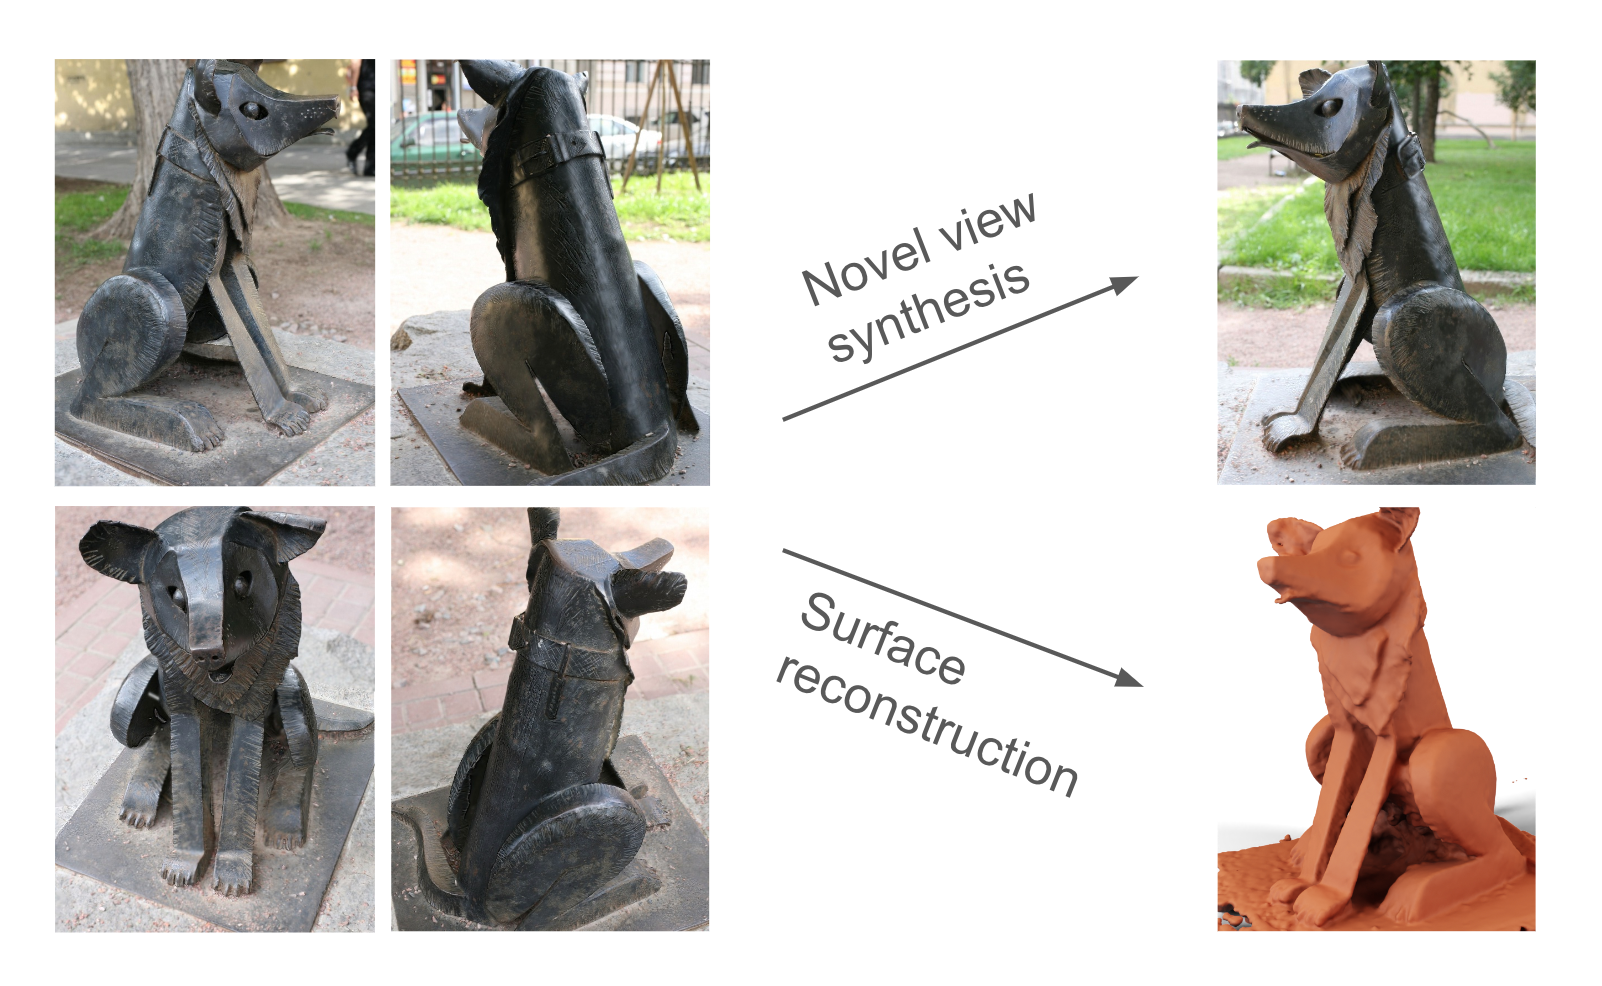
\includegraphics[width=\linewidth]{figures/intro/3d_recon.png}
        \caption{Dog scene from the Blended MVS dataset}
    \end{figure}
\end{frame}

{
\setbeamertemplate{frame footer}{\citet{berkeley_slides}}
\begin{frame}{Traditional Methods}
    \begin{itemize}
        \item Structure from motion
              \begin{figure}
                  \centering
                  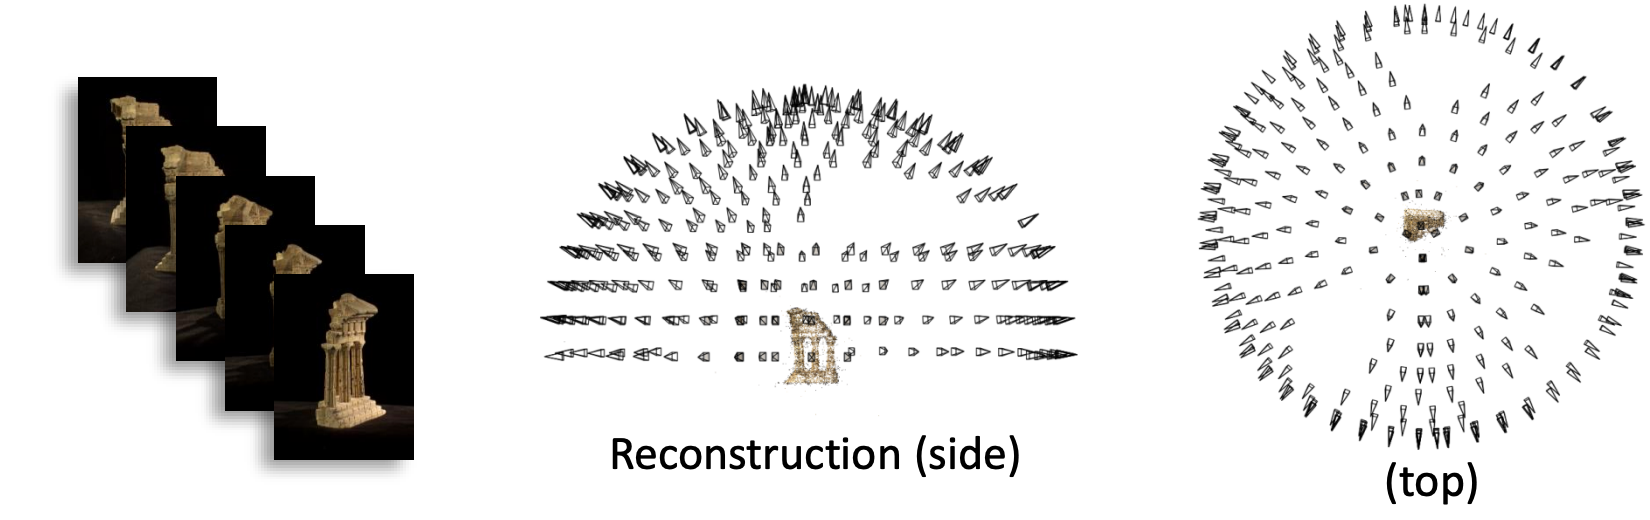
\includegraphics[width=0.7\linewidth]{figures/intro/sfm.png}
              \end{figure}
        \item Multi-view stereo
              \begin{figure}
                  \centering
                  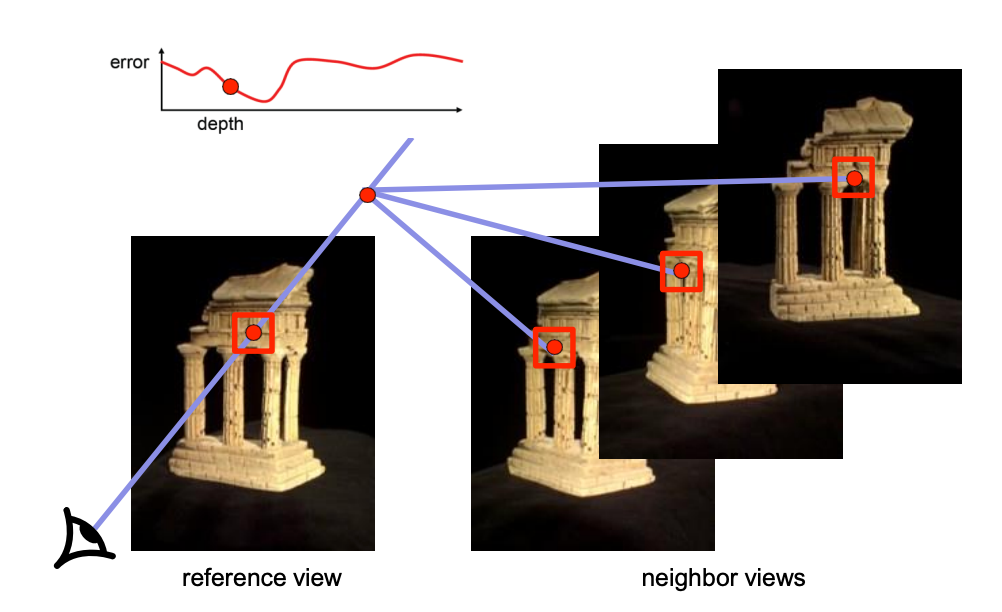
\includegraphics[width=0.6\linewidth]{figures/intro/mvs.png}
              \end{figure}
    \end{itemize}
\end{frame}
}


\begin{frame}{Traditional Methods}
    What do the outputs look like?

    \begin{figure}
        \centering
        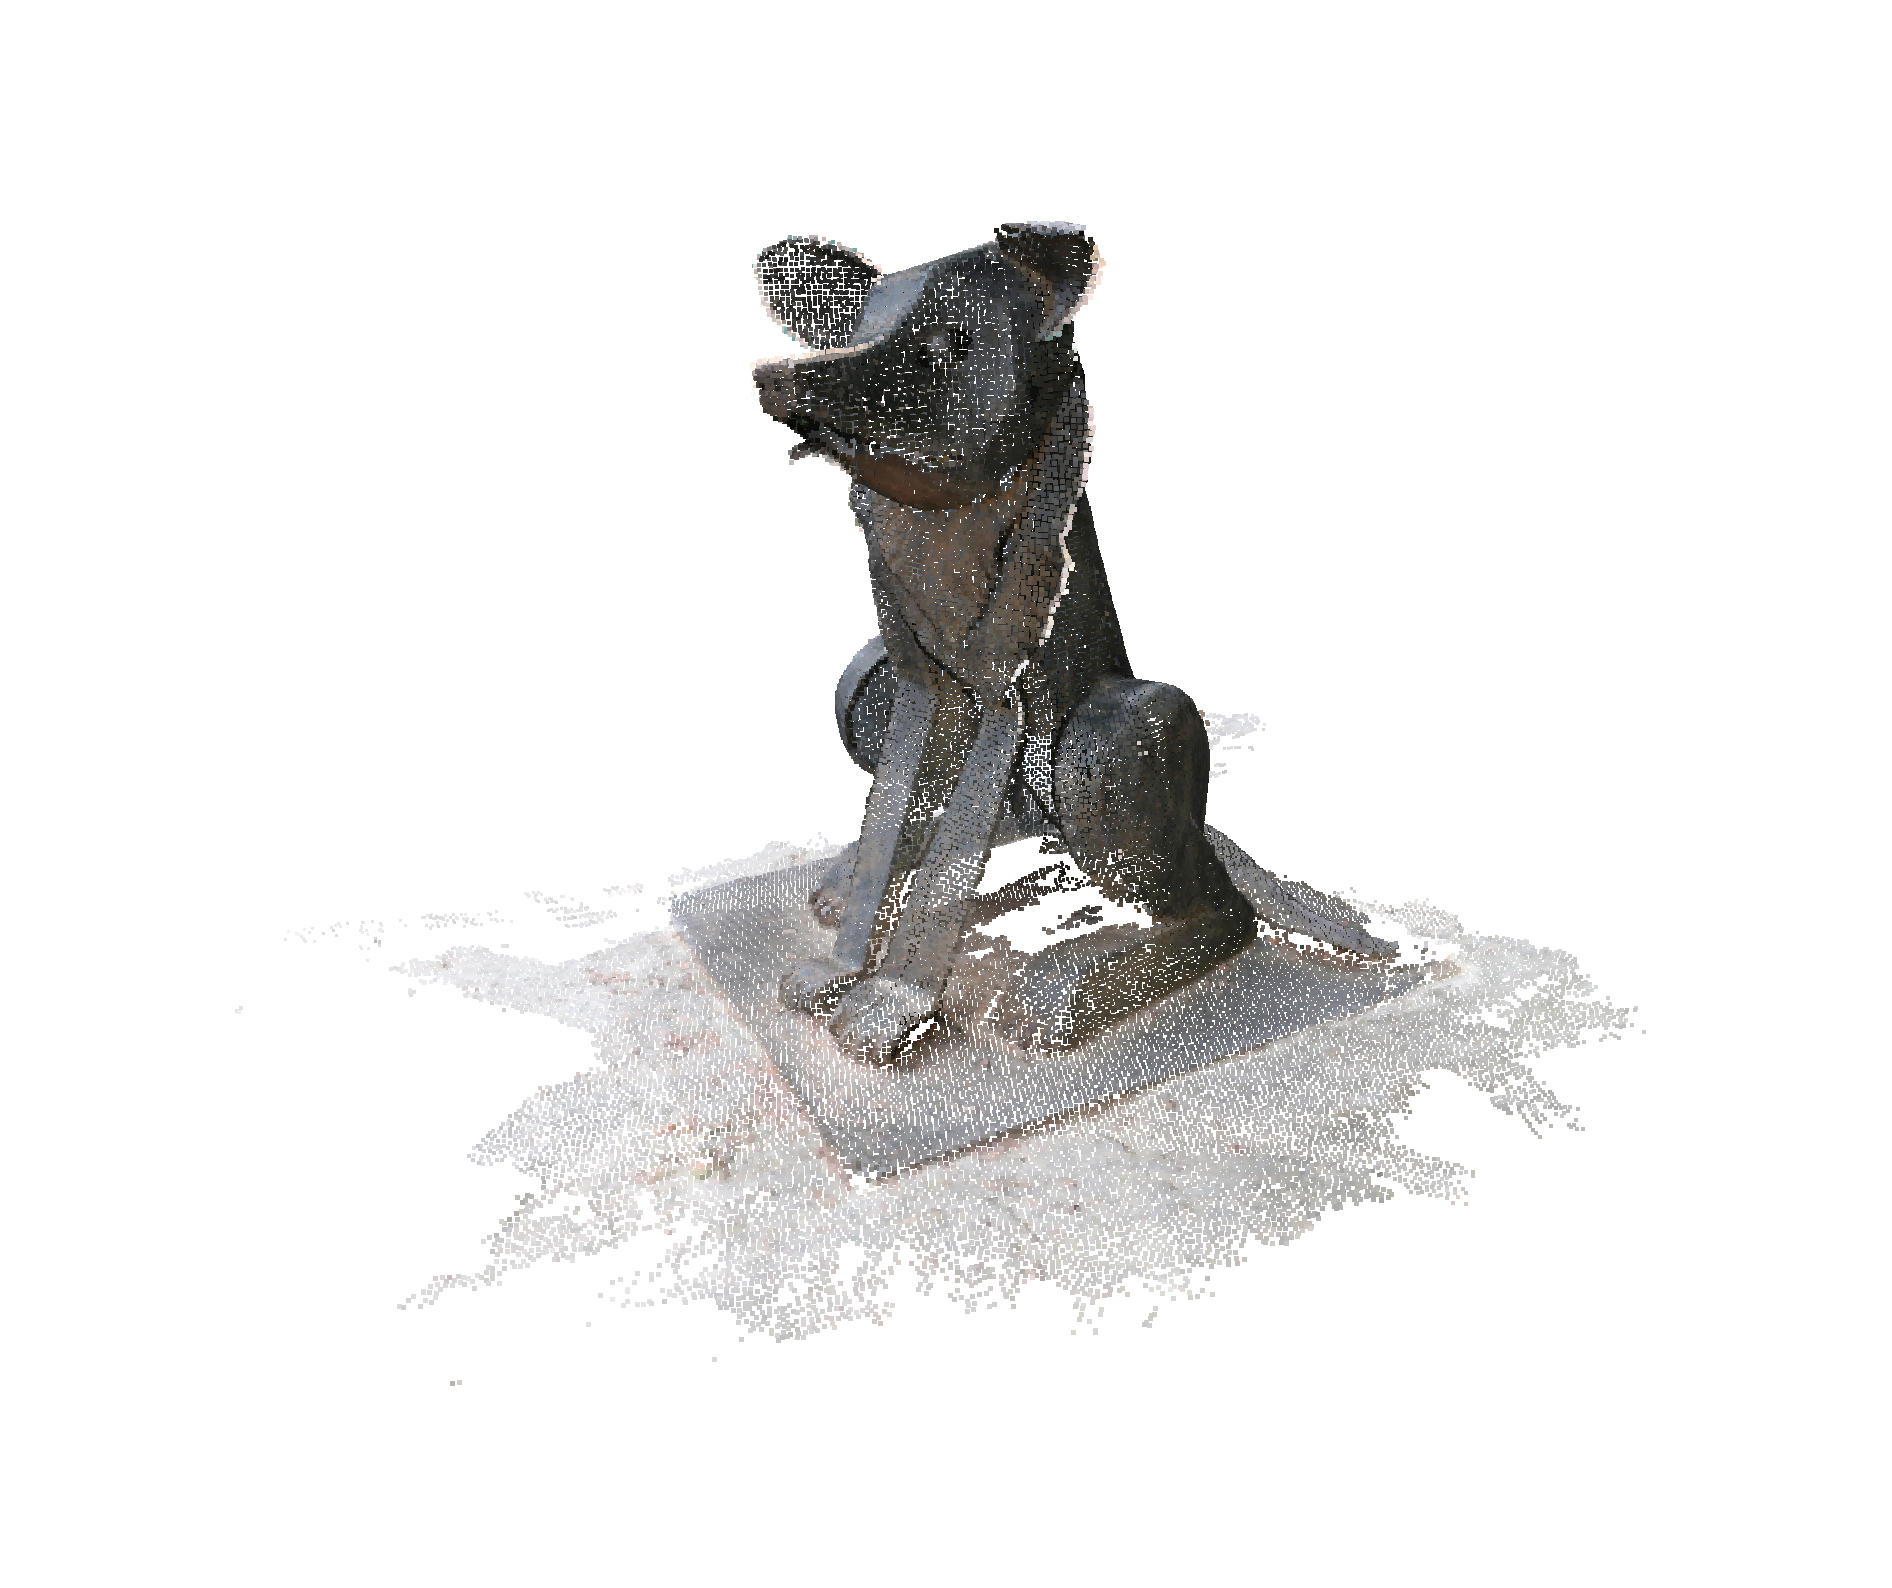
\includegraphics[width=0.6\linewidth]{figures/intro/point_cloud.png}
    \end{figure}
\end{frame}

\begin{frame}{Traditional Methods}
    Looks pretty good, except...

    \begin{figure}
        \centering
        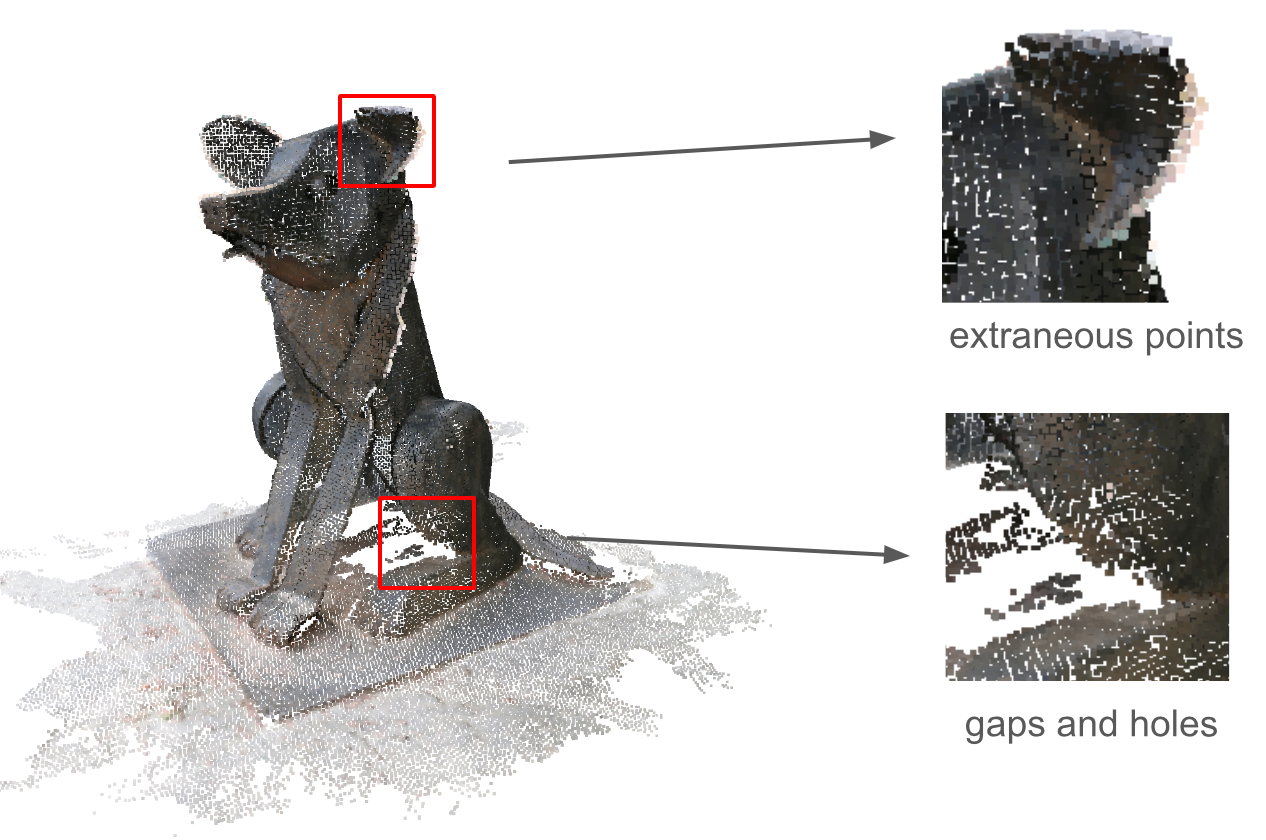
\includegraphics[width=0.8\linewidth]{figures/intro/issues.png}
    \end{figure}
\end{frame}

\begin{frame}{Traditional Methods}
    Typically, \alert{Poisson surface reconstruction} \citep{kazhdan2006poisson} is used to extract surfaces.

    \begin{figure}
        \centering
        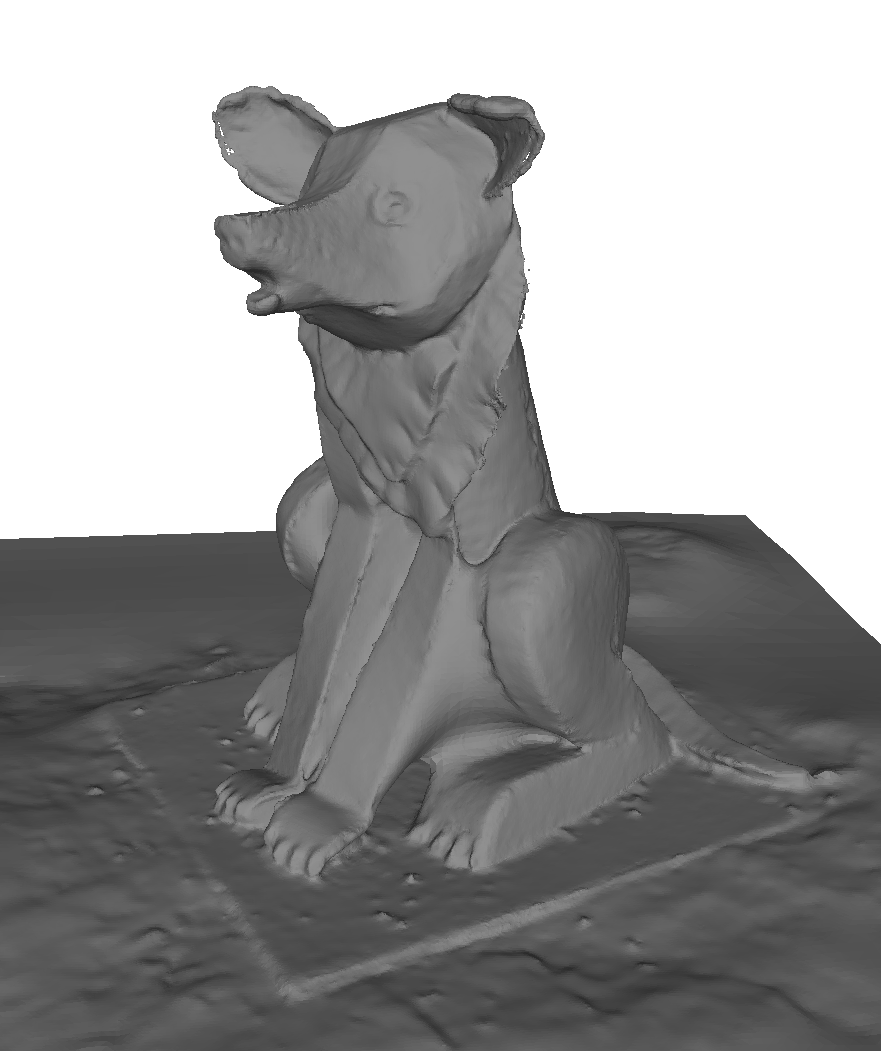
\includegraphics[width=0.5\linewidth]{figures/intro/psr.png}
    \end{figure}
\end{frame}

\begin{frame}{Traditional Methods}
    ... and we see the same issues
    \begin{figure}
        \centering
        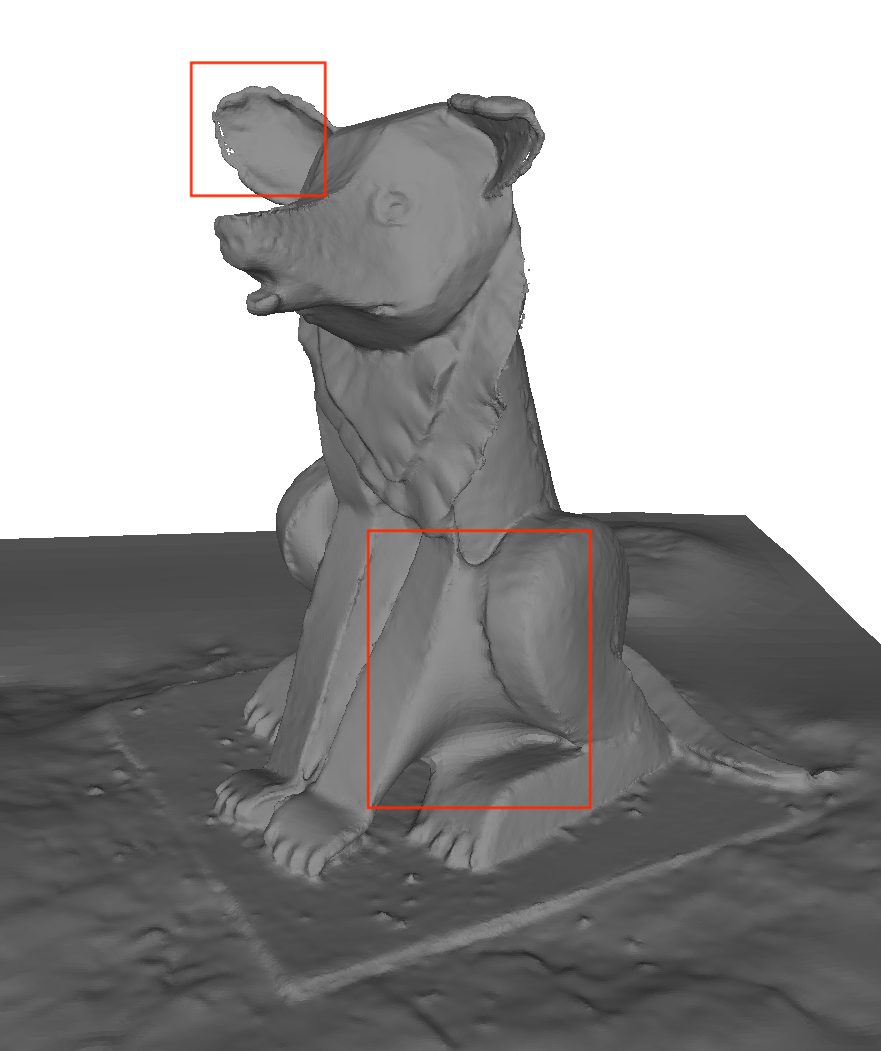
\includegraphics[width=0.5\linewidth]{figures/intro/psr_issues.png}
    \end{figure}
\end{frame}

\section{Volumetric Neural Rendering}

 {
  \setbeamertemplate{frame footer}{\citet{bunny_mesh, Park_2019_CVPR}}
  \begin{frame}{Surface Rendering}
      \begin{figure}
          \centering
          \subfloat[Triangle mesh]{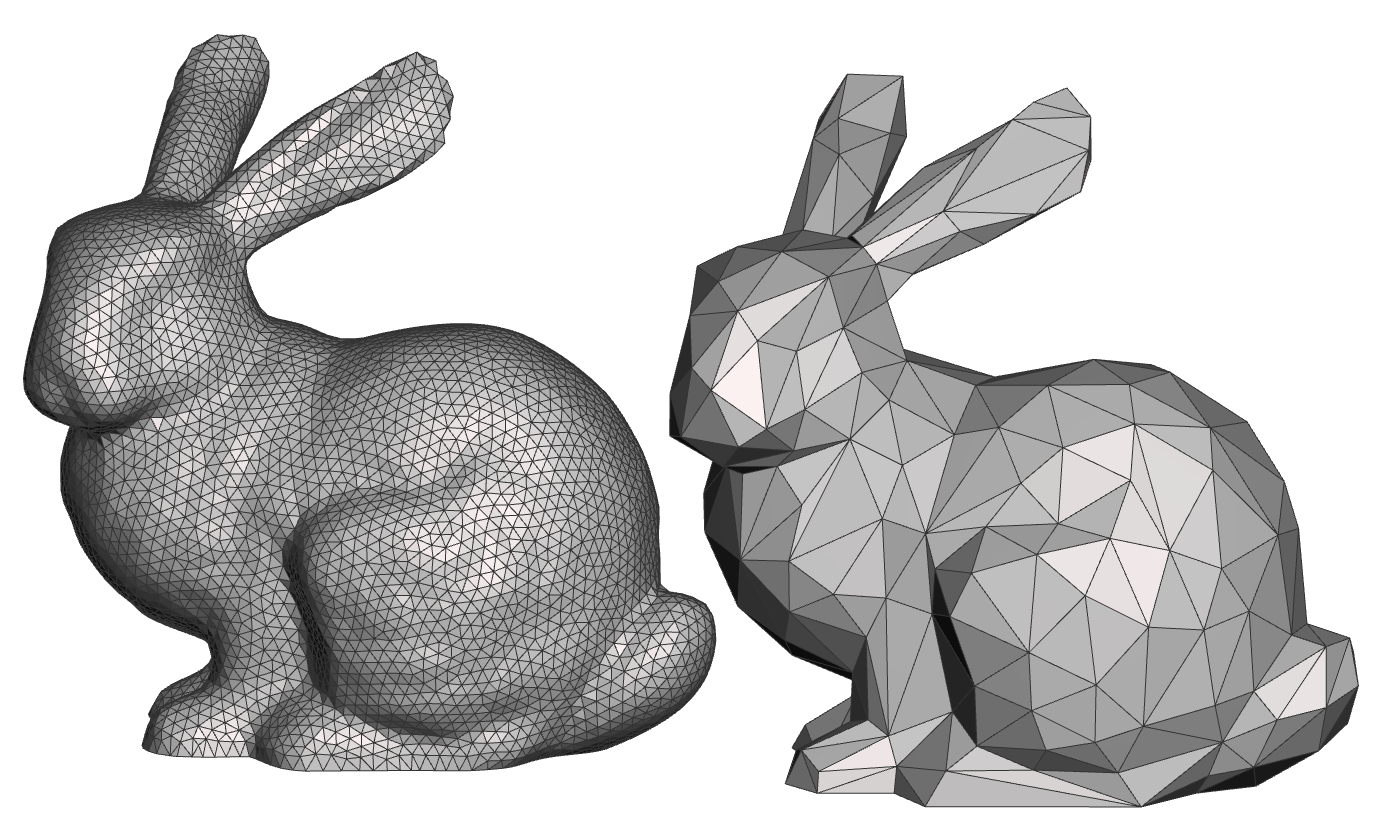
\includegraphics[width=0.45\linewidth]{figures/vol/mesh.png}}\hspace{3em}
          \subfloat[Signed-distance function]{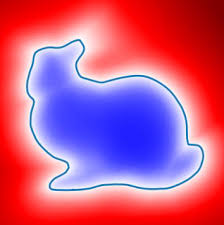
\includegraphics[width=0.35\linewidth]{figures/vol/sdf.jpg}}
      \end{figure}
  \end{frame}
 }

 {
  \setbeamertemplate{frame footer}{\citet{bitterli18framework, rte}}
  \begin{frame}{Volume Rendering}
      \begin{figure}
          \centering
          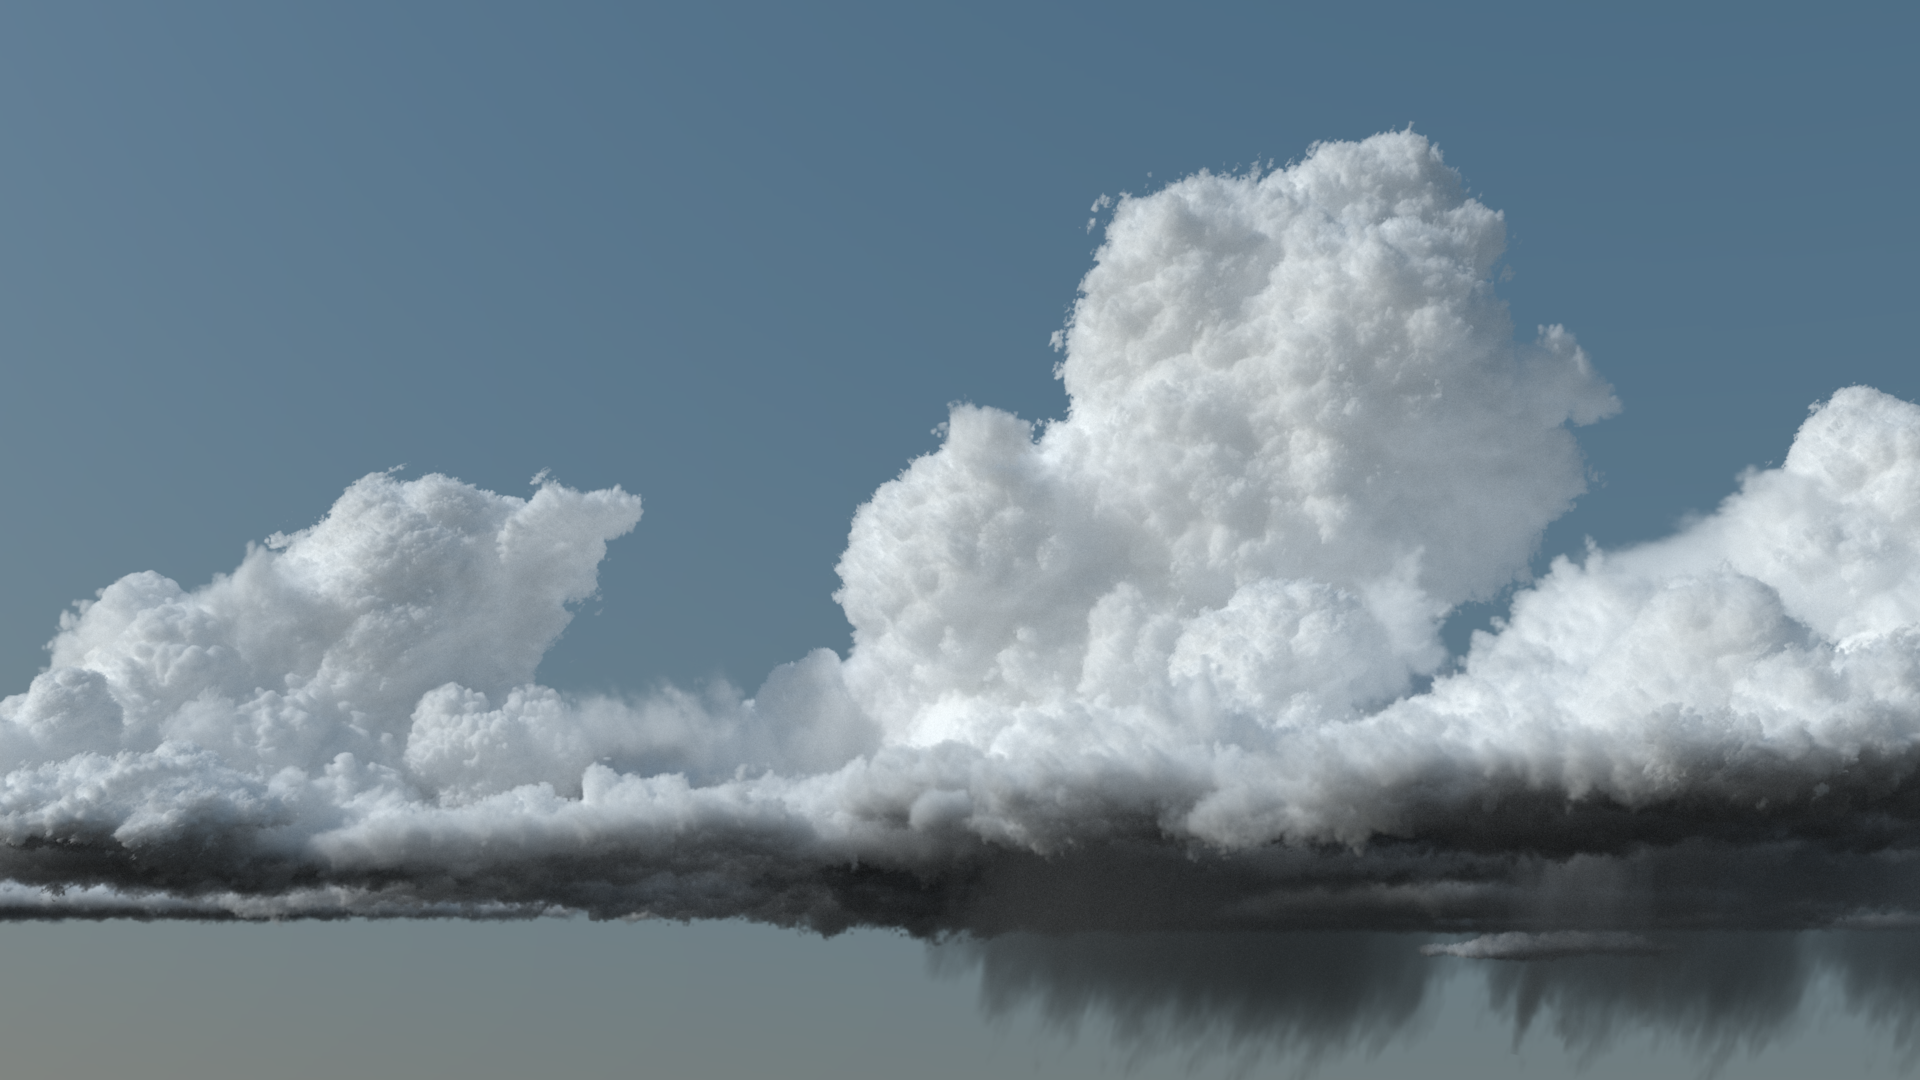
\includegraphics[width=0.6\linewidth]{figures/vol/volume.png} \\ \vspace{0.5em}
          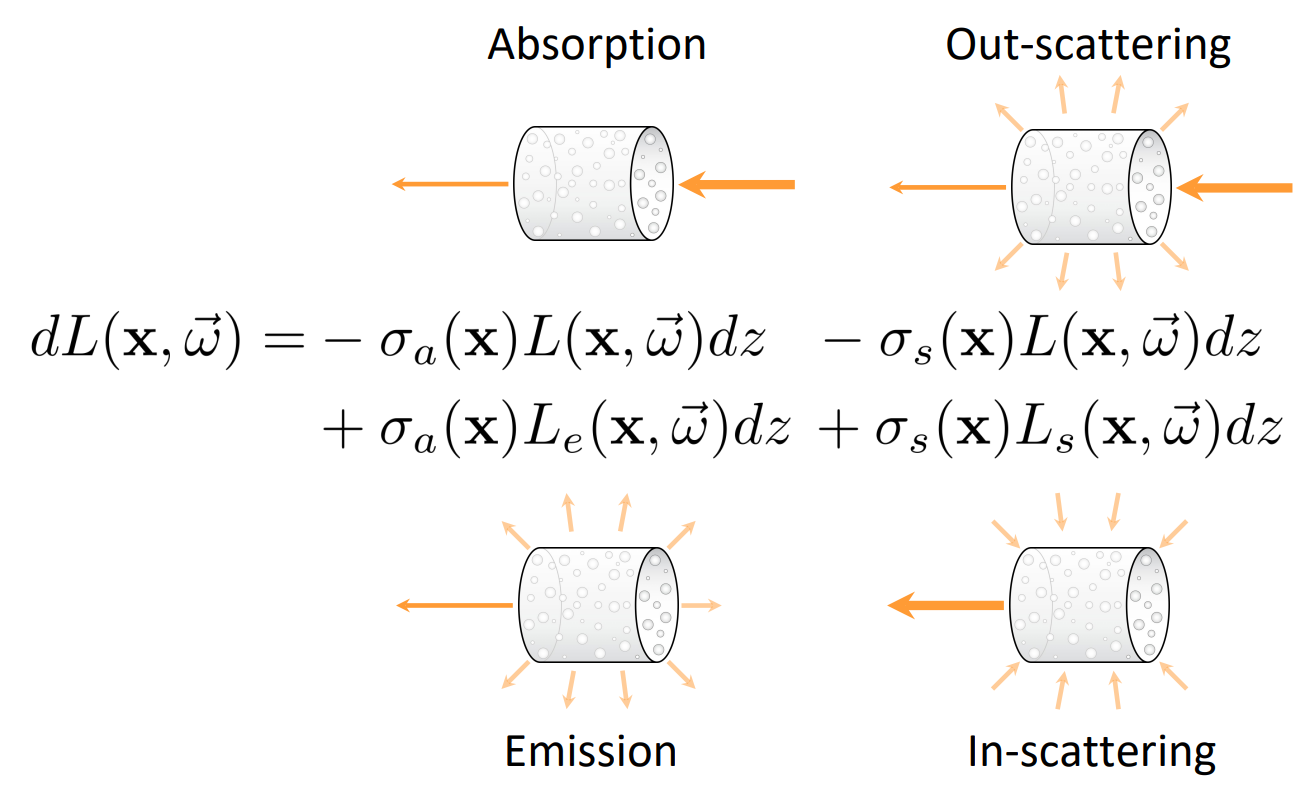
\includegraphics[width=0.5\linewidth]{figures/vol/rte.png}
      \end{figure}
  \end{frame}
 }

\begin{frame}{Rendering Equation}
    Assuming an \emph{emissive} volume with no scattering, we can derive the \alert{rendering equation} as
    \begin{equation*}
        L(\bx, \vec{\omega}) = \int_0^z \mathrm{Tr}(\bx, \bx_t) \sigma(\bx_t, \vec{\omega}) L_e(\bx_t, \vec{\omega})  \; \mathrm{d}t,
    \end{equation*}
    where \(\mathrm{Tr}(\bx, \bx_t)\) is the \alert{transmittance}
    \begin{equation*}
        \mathrm{Tr}(\bx, \bx_t) = \exp\left(-\int_0^t \sigma(\bx_s, \vec{\omega}) \;\mathrm{d}s\right),
    \end{equation*}
    and \(\sigma(\bx_s, \vec{\omega})\) is the spatially varying \alert{attenuation coefficient}.
\end{frame}

{
\setbeamertemplate{frame footer}{\citep{mildenhall2020nerf}}
\begin{frame}{Neural Radiance Fields (NeRF)}
    Representing objects as volumes (instead of surfaces).
    \begin{figure}
        \centering
        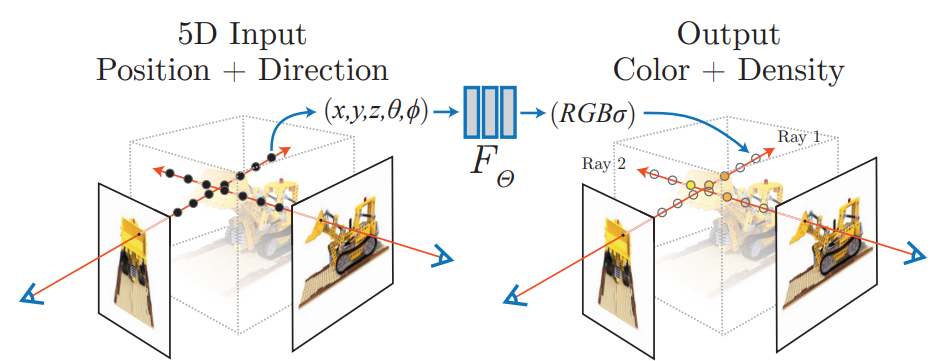
\includegraphics[width=0.9\linewidth]{figures/vol/nerf.png}
    \end{figure}

    Color \(L_e(\bx, \vec{\omega})\) and density \(\sigma(\bx, \vec{\omega})\) modeled by a \alert{neural network}.
\end{frame}

\begin{frame}{Neural Radiance Fields (NeRF)}
    NeRFs work particularly well for \alert{novel-view synthesis} tasks \\

    ... but not so much for \alert{surface extraction}.

    \begin{figure}
        \centering
        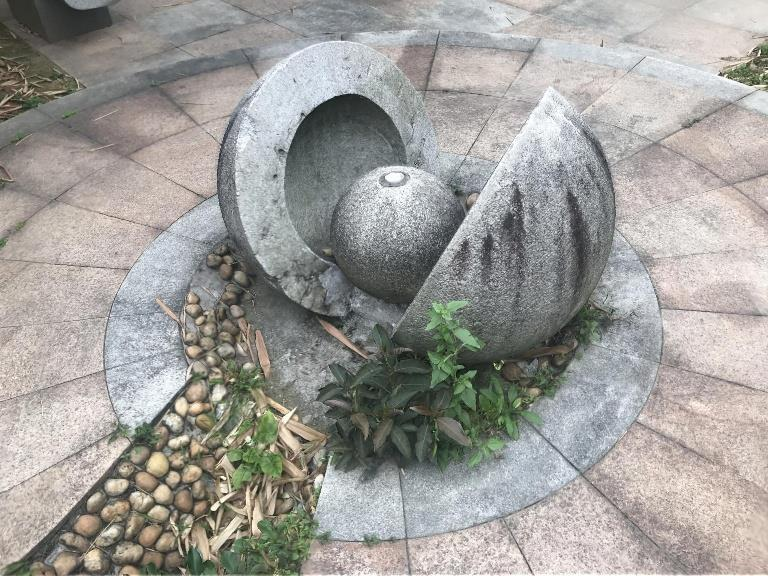
\includegraphics[width=0.35\linewidth]{figures/vol/nerf_surface/143.jpg}
        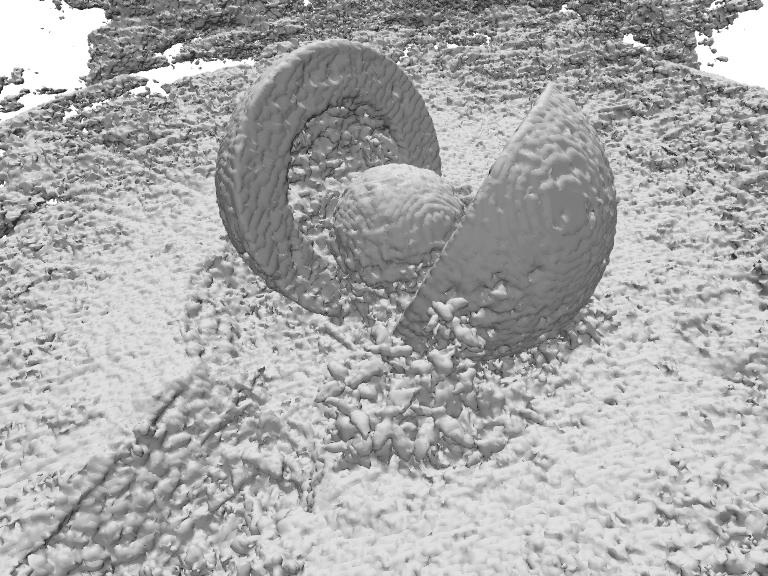
\includegraphics[width=0.35\linewidth]{figures/vol/nerf_surface/1.png} \\ \vspace{0.1em}
        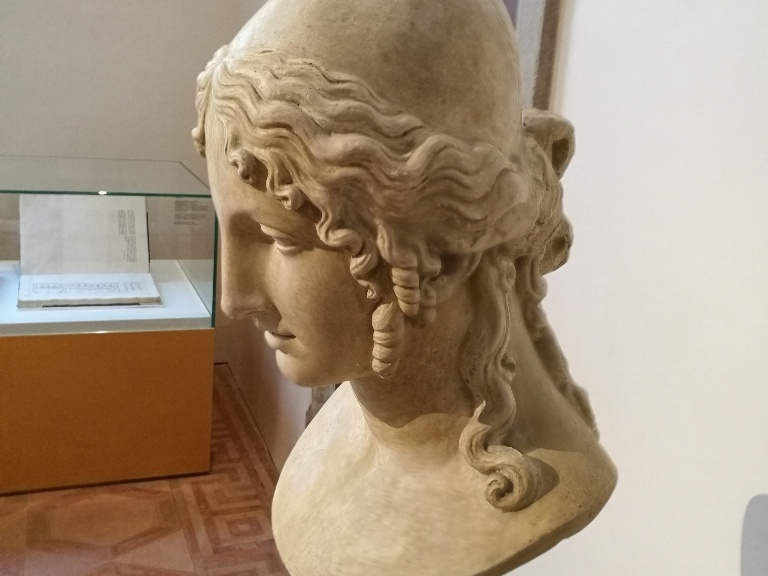
\includegraphics[width=0.35\linewidth]{figures/vol/nerf_surface/32.jpg}
        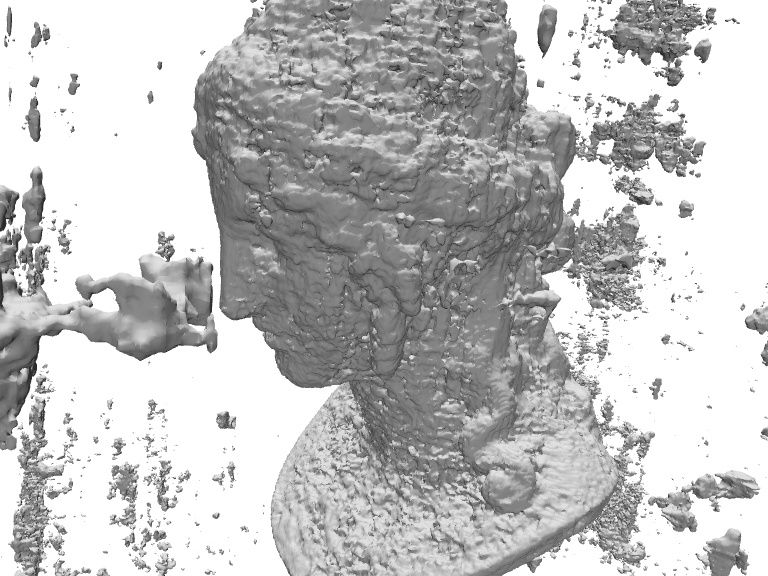
\includegraphics[width=0.35\linewidth]{figures/vol/nerf_surface/2.png}
    \end{figure}
\end{frame}
}

\begin{frame}{Neural Surface Representations}
    Can we explicitly model the \alert{geometry} of the scene?

    Yes, there are many works that already do this:
    \begin{itemize}
        \item Occupancy \(\leftrightarrow\) density {\tiny (NeuS \citep{wang2021neus})}
        \item Signed-distance function \(\leftrightarrow\) density {\tiny (VolSDF \citep{yariv2021volume})}
    \end{itemize}

    Follow-up works improve reconstruction quality and efficiency:
    \begin{itemize}
        \item Multi-resolution hash grids {\tiny (Neuralangelo \citep{li2023neuralangelo}, NeuS2 \citep{neus2})}
        \item Photo-consistency constraints {\tiny (Neuralwarp \citep{neuralwarp}, Geo-NeuS \citep{Fu2022GeoNeus})}
        \item Sparse voxel representation {\tiny (Voxurf \citep{wu2022voxurf})}
    \end{itemize}
\end{frame}

\begin{frame}{Neural Surface Representations}
    Limitations of existing methods:
    \begin{itemize}
        \item Trade-off between speed and reconstruction quality
        \item Cannot effectively leverage \alert{known information}
    \end{itemize}

    Our solution: Directly build off of the output of traditional methods (i.e. dense \alert{point clouds})
\end{frame}

\section{Winding Number \& Dipole Sums}

 {
  \setbeamertemplate{frame footer}{\citet{wn,Barill:FW:2018}}
  \begin{frame}{The Winding Number}
      \begin{figure}
          \centering
          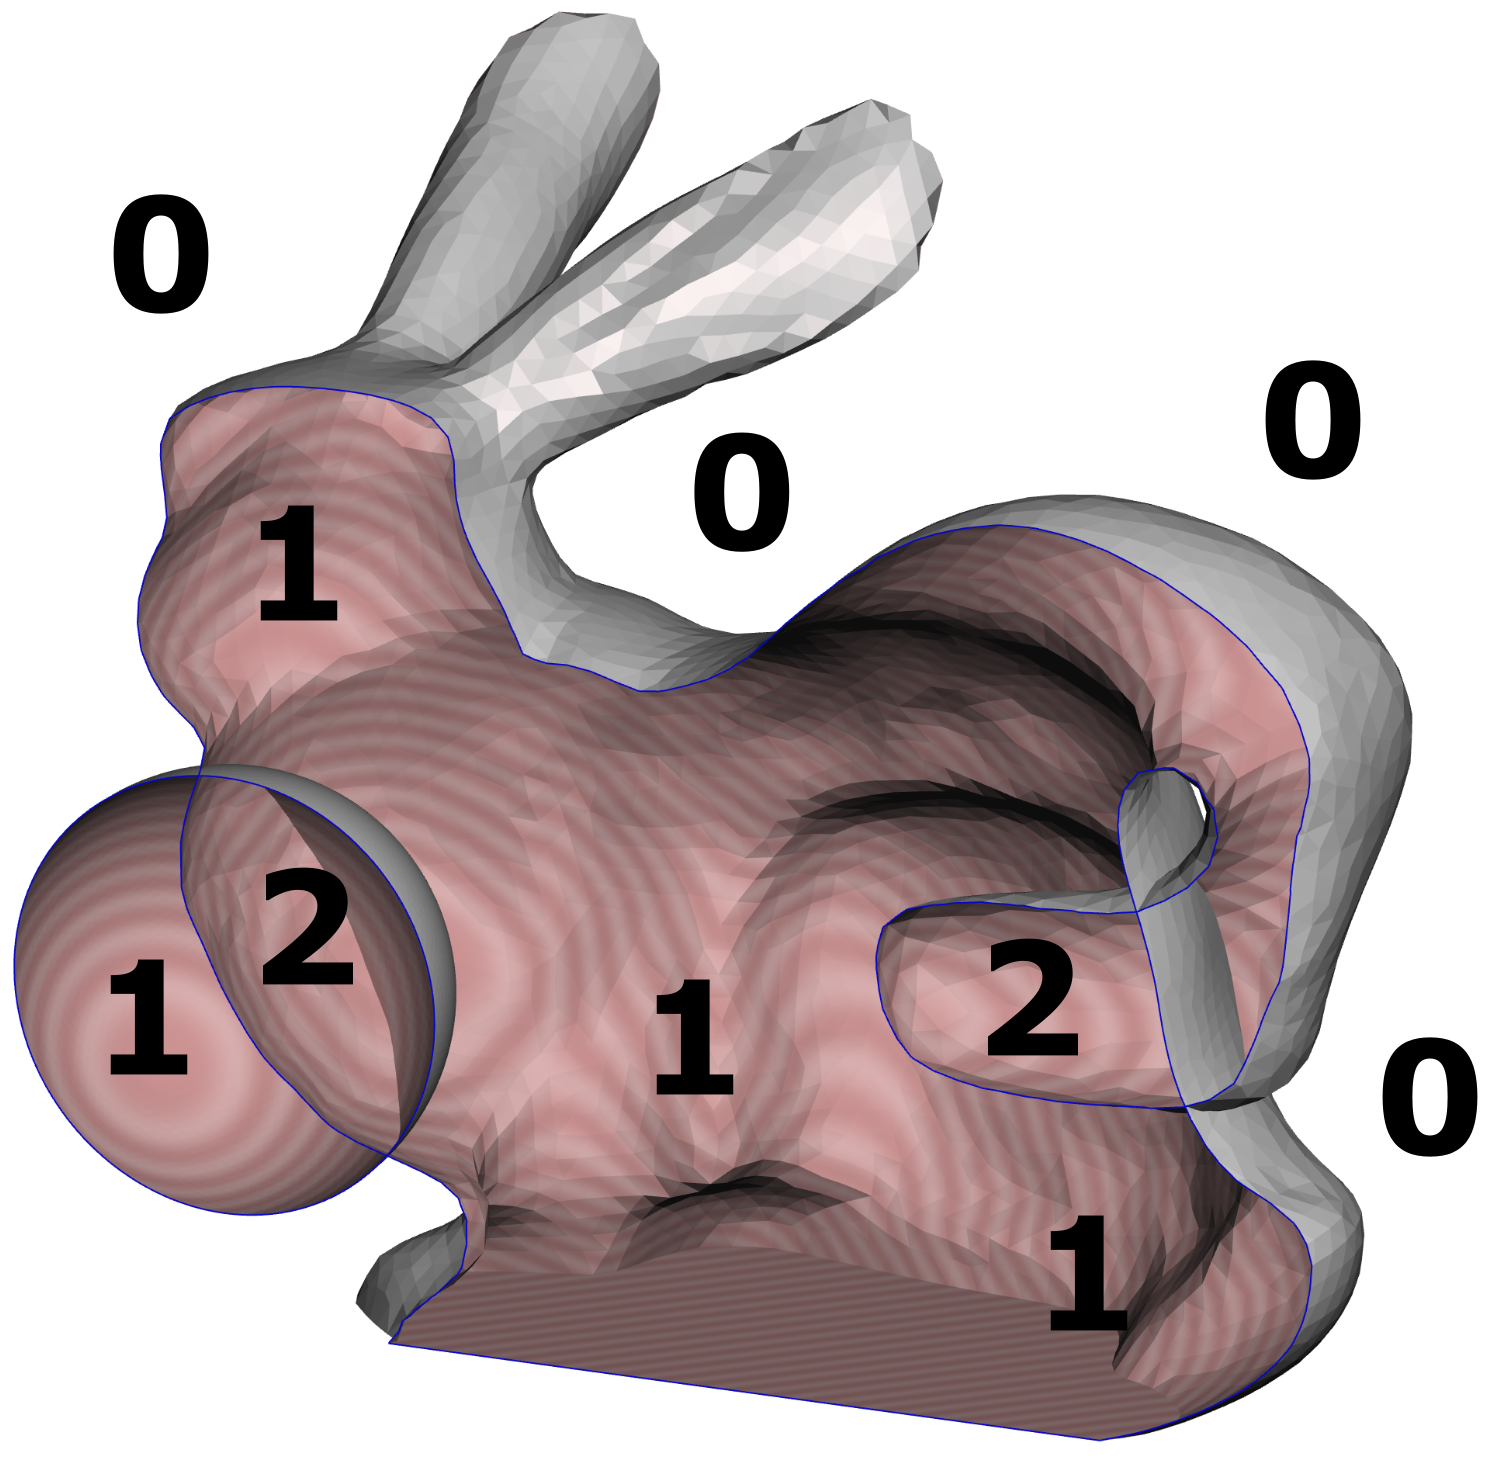
\includegraphics[width=0.4\linewidth]{figures/wn/wn.png}
      \end{figure}

      \begin{equation*}
          w_S(\bq) = \frac{1}{4\pi} \int_{S} \mathrm{d}\Omega(\bq) = \int_{S} \frac{(\bp - \bq) \cdot \widehat{\bn}}{4\pi \|\bp - \bq\|^3} \; \mathrm{d}\bp
      \end{equation*}
  \end{frame}
 }

 {
  \setbeamertemplate{frame footer}{\citet{Barill:FW:2018}}
  \begin{frame}{The \alert{Generalized} Winding Number}
      \begin{figure}
          \centering
          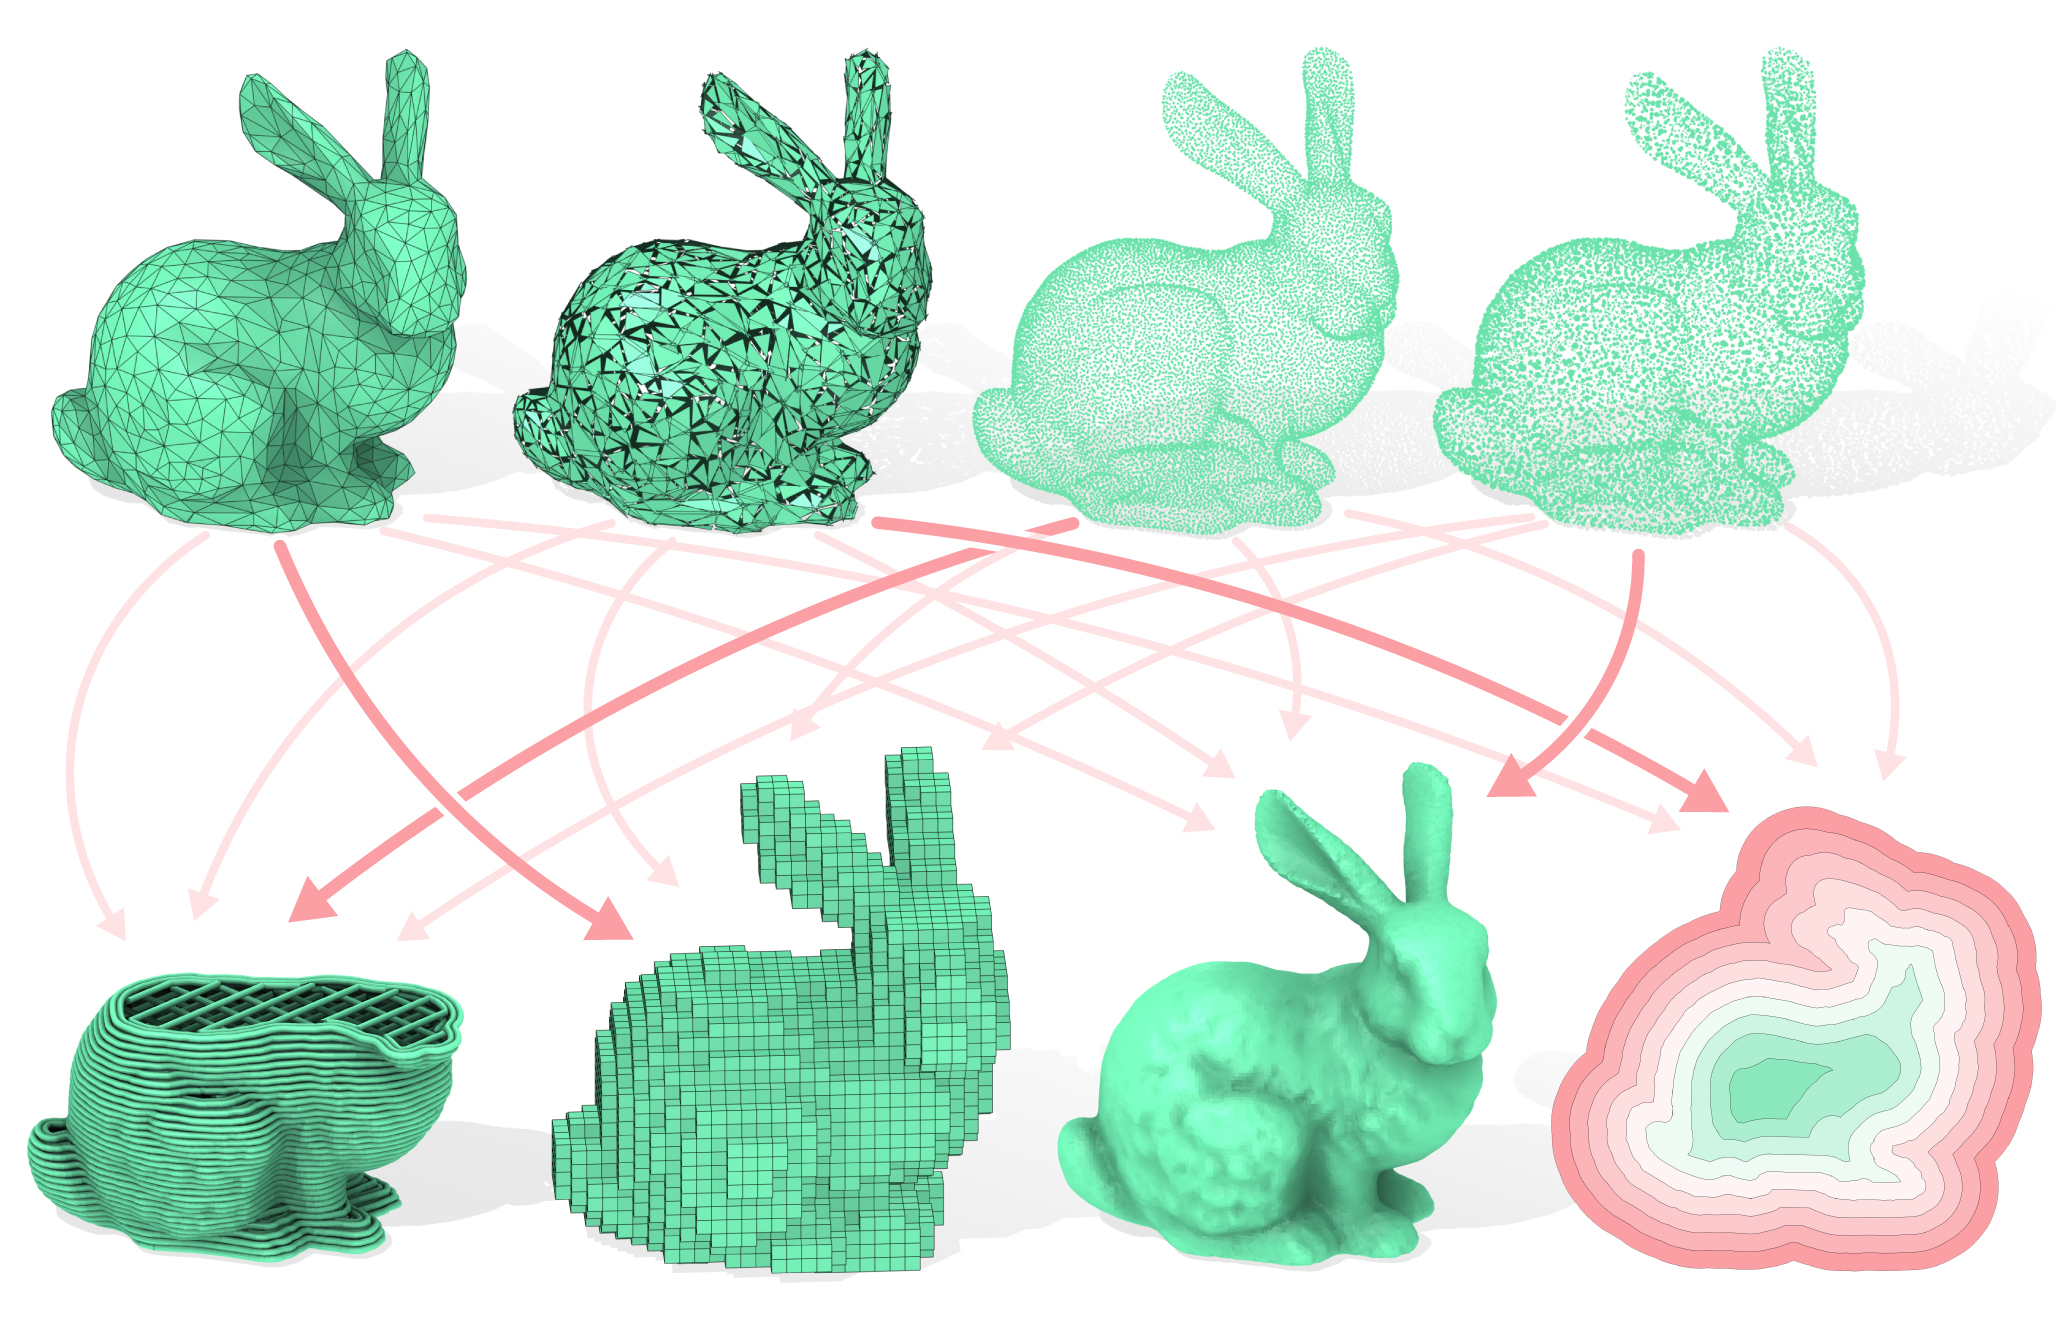
\includegraphics[width=0.6\linewidth]{figures/wn/gwn.png}
      \end{figure}

      For point clouds,
      \begin{equation*}
          w_S(\bq) \approx \sum_{m=1}^{N} a_m \frac{(\bp_m - \bq)\cdot \widehat{\bn}_m}{4\pi\|\bp_m - \bq\|^3}
      \end{equation*}
      where \(a_m\) are ``area-weights'' (e.g. geodesic Voronoi area).
  \end{frame}
 }


\begin{frame}{The \alert{Generalized} Winding Number}
    \begin{figure}
        \centering
        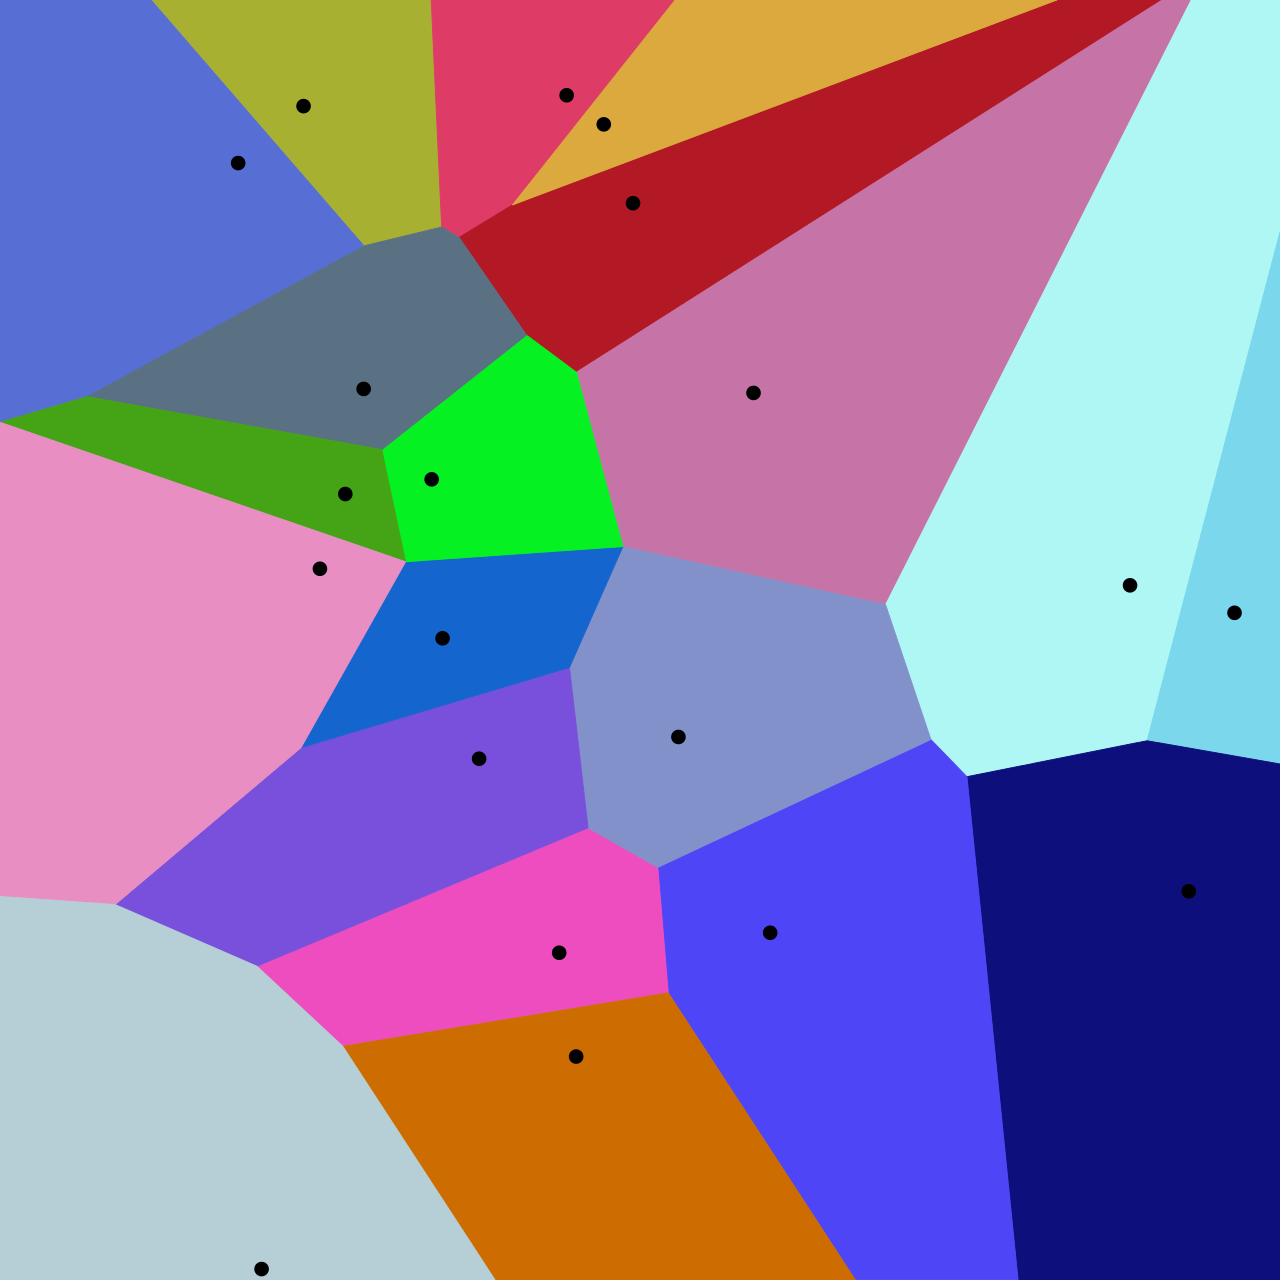
\includegraphics[width=0.5\linewidth]{figures/wn/voronoi.png}
    \end{figure}
\end{frame}

\begin{frame}{\alert{Aside}: Laplace BVP}
    The winding numbers are also the solutions to the Laplace boundary value problem (BVP)
    \begin{align*}
        \begin{cases}
            \Delta w(\bp) = 0,                                                                                       & \bp \in {\mathbb R}^3 \backslash \partial \Omega \\
            w^+(\bp) - w^-(\bp) = f(\bp),                                                                            & \bp \in \partial \Omega                          \\
            \frac{\partial w^+}{\partial \widehat{\bn}}(\bp) - \frac{\partial w^-}{\partial \widehat{\bn}}(\bp) = 0, & \bp \in  \partial \Omega,
        \end{cases}
    \end{align*}
    for the case where \(f(\bp) \equiv 1\) on the boundary.
\end{frame}

\begin{frame}{The \alert{Generalized} Winding Number}
    Naively, we can directly extract the \(0.5\)-isosurface of the winding number field. However, this often fails in practice...
    \begin{figure}
        \centering
        \hspace{-2em}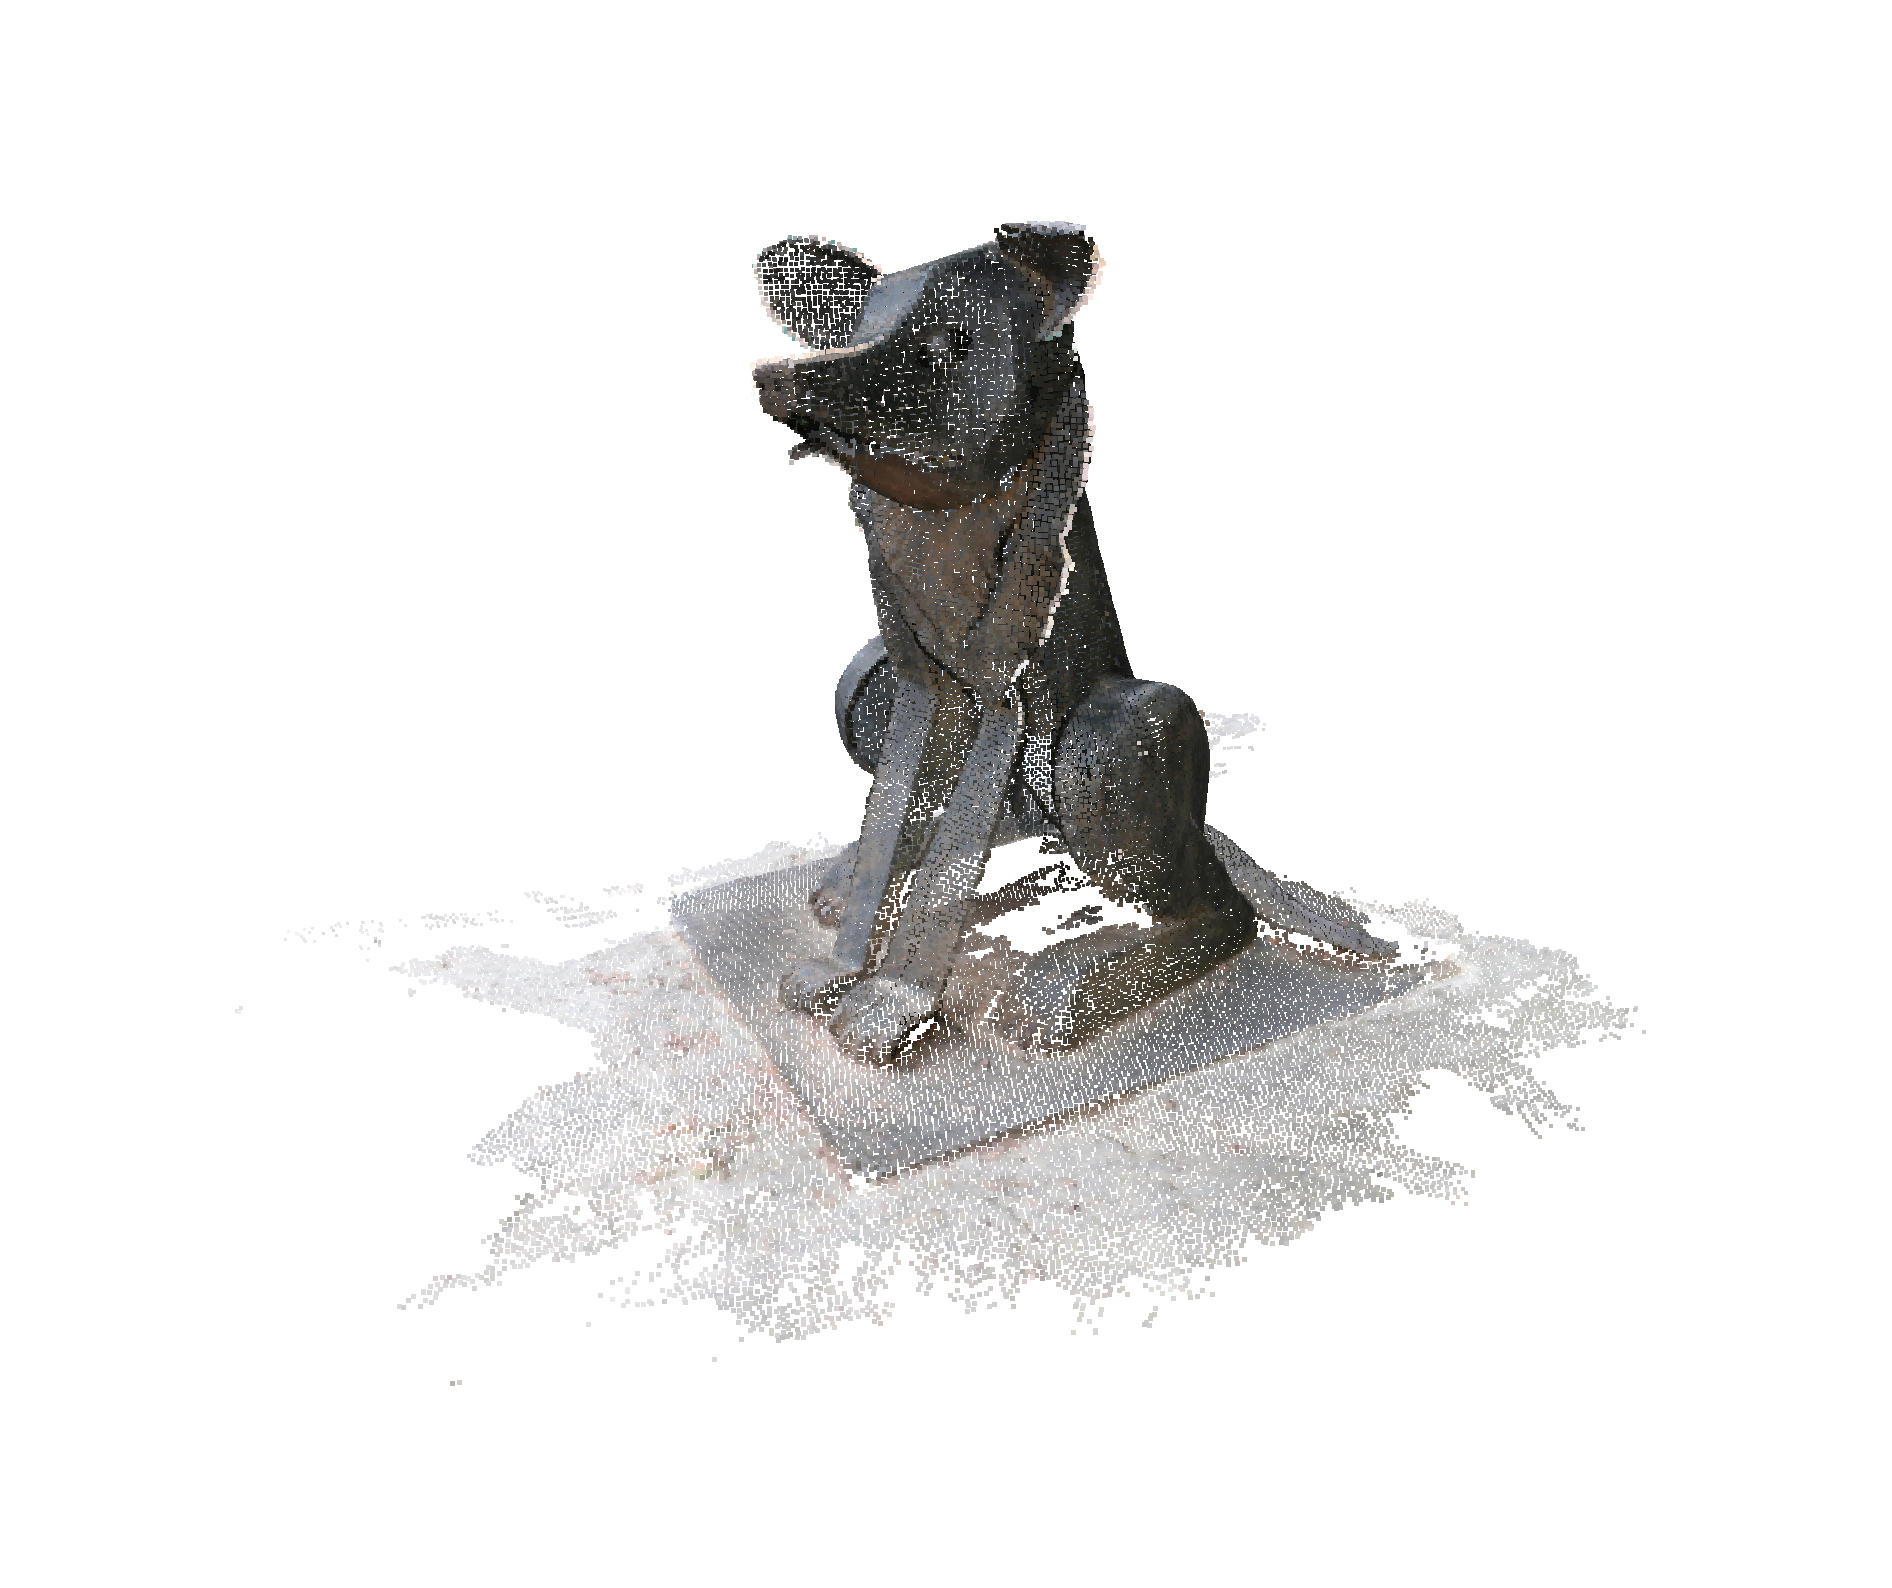
\includegraphics[width=0.48\linewidth]{figures/intro/point_cloud.png}
        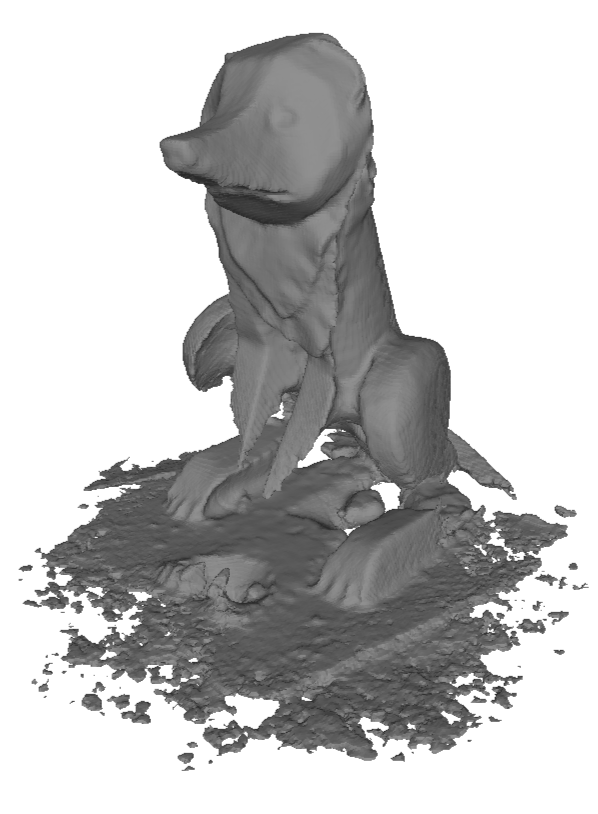
\includegraphics[width=0.3\linewidth]{figures/wn/gwn_mesh.png}
    \end{figure}
\end{frame}


\begin{frame}{The Dipole Sum}
    What if we further generalize the winding number

    ... and allow \(f(\bp) \not\equiv 1\)?
    \begin{align*}
        w_S(\bq) = \int_{S}   & \frac{(\bp - \bq) \cdot \widehat{\bn}}{4\pi \|\bp - \bq\|^3} \cdot 1 \;\mathrm{d}\bp      \\
                              & \Downarrow                                                                                \\
        u^f_S(\bq) = \int_{S} & \frac{(\bp - \bq) \cdot \widehat{\bn}}{4\pi \|\bp - \bq\|^3} \cdot f(\bp) \;\mathrm{d}\bp
    \end{align*}
\end{frame}

\begin{frame}{The Dipole Sum}
    This is equivalent to having non-unit \alert{per-point} attributes \(f_m\):
    \begin{align*}
        w_{\mathrm{pc}}(\bq) = \sum_{m=1}^{N}   & a_m \frac{(\bp_m - \bq)\cdot \widehat{\bn}_m}{4\pi\|\bp_m - \bq\|^3} \cdot 1     \\
                                                & \Downarrow                                                                       \\
        u^f_{\mathrm{pc}}(\bq) = \sum_{m=1}^{N} & a_m \frac{(\bp_m - \bq) \cdot \widehat{\bn}_m}{4\pi \|\bp_m - \bq\|^3} \cdot f_m
    \end{align*}

    In a differentiable rendering pipeline, we can make them learnable!
\end{frame}

\begin{frame}{The \alert{Fast} Dipole Sum}
    A dense point cloud can have \alert{tens of thousands} of points

    ... and to render a single image, we need to potentially query the dipole sum at \alert{billions} of distinct locations in the scene.

    Obviously, we cannot compute the entire sum for every query...
\end{frame}

\begin{frame}{The Barne-Hut Approximation}
    As proposed by \citet{Barill:FW:2018}, we can consider a cluster of points far away from the query point as a single ``dipole'' with attributes computed using the \alert{Barnes-Hut approximation}.

    \begin{figure}
        \centering
        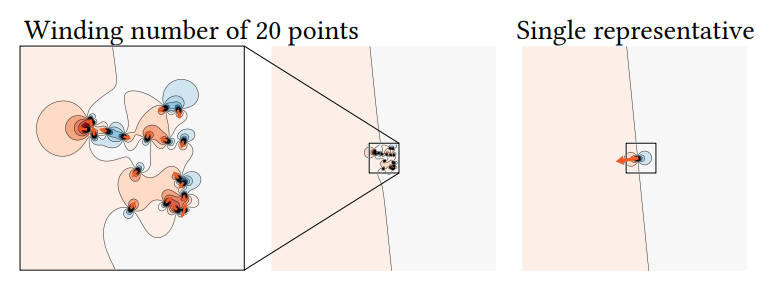
\includegraphics[width=0.9\linewidth]{figures/wn/barne_hut.png}
    \end{figure}
\end{frame}

\begin{frame}{The Barne-Hut Approximation}
    We construct an \alert{octree} from the point cloud, and assign each tree node \(t\) a centroid, a weighted normal, and a radius, computed from its leaves \(\mathcal L(t)\):
    \begin{align*}
        \tilde{\bp}_t   & \equiv \frac{\sum_{m \in \mathcal L(t)} a_m \bp_m}{\sum_{m \in \mathcal L(t)} a_m} \\
        \tilde{\bn}^f_t & \equiv \sum_{m \in \mathcal L(t)} a_m \widehat{\bn}_m \cdot f_m                    \\
        \tilde{r}_t     & \equiv \max_{m \in \mathcal L(t)} \|\tilde{\bp}_t - \bp_m\|
    \end{align*}

    To query the \alert{fast} dipole sum, we recurse the octree with aggressive pruning in \(O(\log N)\) time.
\end{frame}

\begin{frame}{Fast Backpropogation}
    Naively backpropagating through the dipole sum takes \(O(N\cdot M)\) time for \(M\) queries.

    We propose a two-stage backprop scheme:
    \begin{enumerate}
        \item
              We \alert{detach} the per-node parameters from the per-point parameters and \alert{cache} gradients at nodes.
        \item
              We use the \alert{chain rule} to propogate gradients from the nodes to all leaves (points).
    \end{enumerate}

    Each iteration of backprop only takes \(O((M + N)\log N)\) time.
\end{frame}


\section{Rendering}

 {
  \setbeamertemplate{frame footer}{\(^\dagger\) We actually use a \alert{regularized} version of the dipole sum to avoid singularities}
  \begin{frame}{Fast Dipole Sum \(\rightarrow\) Occupancy}
      To convert the dipole sum\(^\dagger\) into \alert{occupancy} values between \(0\) and \(1\), we apply a logistic sigmoid
      \begin{equation*}
          O(\bq) = \frac{1}{1 + \exp\left(-s\cdot (u^f_\mathrm{pc}(\bq) - 0.5)\right)}
      \end{equation*}
      with a learnable scale parameter \(s\).

      \begin{figure}
          \centering
          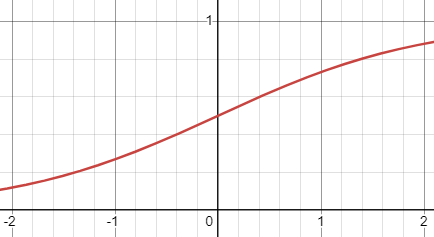
\includegraphics[width=0.4\linewidth]{figures/wn/sigmoid_1.png}\hspace{1em}
          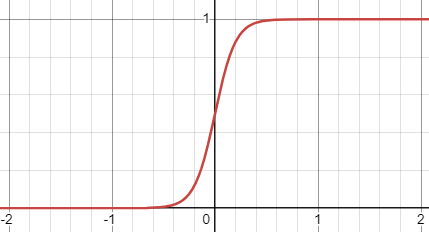
\includegraphics[width=0.4\linewidth]{figures/wn/sigmoid_10.png}
      \end{figure}
  \end{frame}
 }

\begin{frame}{Occupancy \(\rightarrow\) Density}
    To convert the occupancy into \alert{density} (attenuation coefficient) values, we follow \citet{Miller:VOS:2023}:
    \begin{equation*}
        \sigma(\bq, \vec{\omega}) = \frac{|\nabla O(\bq) \cdot \vec{\omega}|}{1 - O(\bq)}
    \end{equation*}

    Intuitively, we have
    \begin{center}
        \begin{tabular}{c|c|c}
            \(\sigma(\bq, \vec{\omega})\) & High             & Low             \\
            \hline
            \(O(\bq)\)                    & High             & Low             \\
            \(\nabla O(\bq)\)             & Large magnitude  & Small magnitude \\
            \(\vec{\omega}\)              & Normal incidence & Grazing angle
        \end{tabular}
    \end{center}
\end{frame}

\begin{frame}{Neural Features}
    We can also use the dipole sum as an \alert{interpolation} scheme to interpolate per-point \alert{neural features} \(\bl_m \in \mathbb R^d\):
    \begin{equation*}
        u^\bl_{\mathrm{pc}}(\bq) = \sum_{m=1}^{N} a_m \frac{(\bp_m - \bq) \cdot \widehat{\bn}_m}{4\pi \|\bp_m - \bq\|^3} \cdot \bl_m
    \end{equation*}

    Unlike for geometry, we do not want sharp discontinuities in the interpolated features, so in practice, we instead use
    \begin{equation*}
        u^\bl_{\mathrm{pc}}(\bq) = \sum_{m=1}^{N} a_m \frac{1}{4\pi \|\bp_m - \bq\|^2} \cdot \bl_m
    \end{equation*}
\end{frame}


\begin{frame}{Neural Features}
    We predict colors using a simple neural network
    \begin{equation*}
        L_e(\bq, \vec{\omega}) \approx \mathrm{NN}(u^\bl_{\mathrm{pc}}(\bq), \mathrm{Enc}(\vec{\omega}))
    \end{equation*}
    with a directional encoding function that encodes the viewing direction using spherical harmonics, following \citet{verbin2022refnerf}.
\end{frame}

\section{Results}

\begin{frame}{Setup}
    We implement our method in PyTorch based on the NeuS codebase \citep{wang2021neus}. Dipole sum and octree operations are implemented in C++ and CUDA with PyTorch bindings.

    We evaluate our method against Neuralangelo \citep{li2023neuralangelo} on the DTU dataset \citep{jensen2014large} and BlendedMVS dataset \citep{yao2020blendedmvs} on a single NVIDIA RTX4090 GPU. Each scene takes around 3-4 hours to fully train.
\end{frame}

{
\setbeamertemplate{frame footer}{\(^\dagger\) We exclude scans 63, 83, 105 from the mean calculation due to inaccurate ground truths.}
\begin{frame}{Results: \alert{DTU}}
    We quantitatively evaluate our method on the DTU dataset using the Chamfer distance metric \((\downarrow)\).
    \begin{table}[!htp]
        \scriptsize
        \centering
        \begin{tabular}{lrr}
            \toprule
            Scan             & Ours          & Neuralangelo  \\
            \hline
            24               & 0.46          & \textbf{0.37} \\
            37               & \textbf{0.65} & 0.72          \\
            40               & \textbf{0.33} & 0.35          \\
            55               & \textbf{0.33} & 0.35          \\
            63               & 0.95          & \textbf{0.87} \\
            65               & 0.78          & \textbf{0.54} \\
            69               & \textbf{0.53} & \textbf{0.53} \\
            83               & \textbf{1.23} & 1.29          \\
            97               & \textbf{0.84} & 0.97          \\
            105              & \textbf{0.70} & 0.73          \\
            106              & \textbf{0.46} & 0.47          \\
            110              & \textbf{0.55} & 0.74          \\
            114              & 0.33          & \textbf{0.32} \\
            118              & \textbf{0.37} & 0.41          \\
            122              & \textbf{0.36} & 0.43          \\
            Mean\(^\dagger\) & \textbf{0.50} & 0.52          \\
            \bottomrule
        \end{tabular}
    \end{table}
\end{frame}
}

\begin{frame}{Results: \alert{BlendedMVS}}
    Qualitative equal-time comparisons on the BlendedMVS dataset:
    \begin{figure}
        \centering
        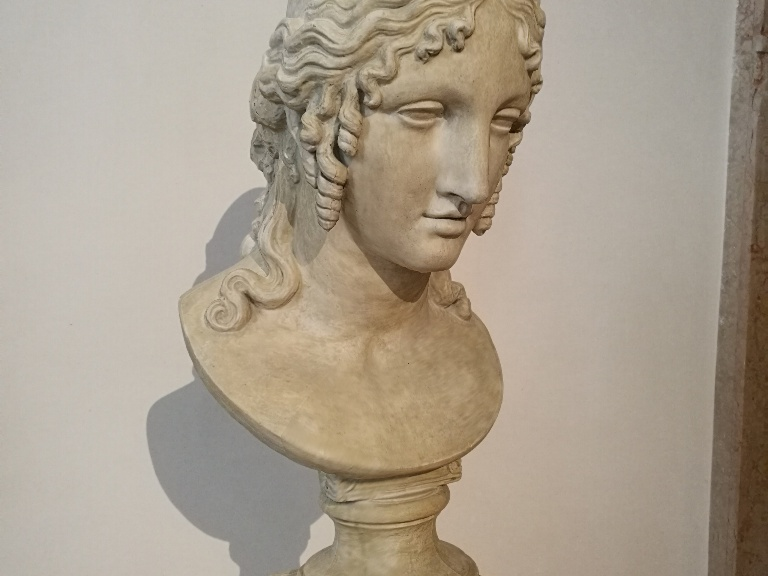
\includegraphics[width=0.3\linewidth]{figures/results/sculpture.png}
        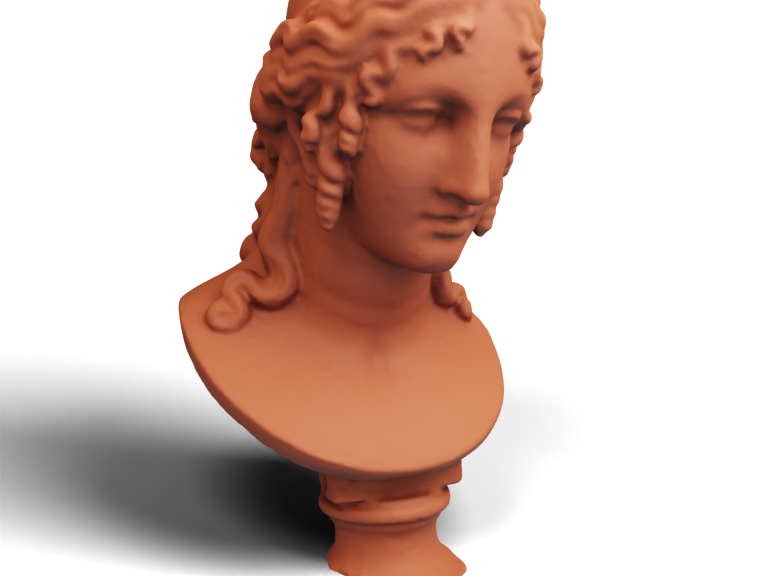
\includegraphics[width=0.3\linewidth]{figures/results/sculpture_ours.png}
        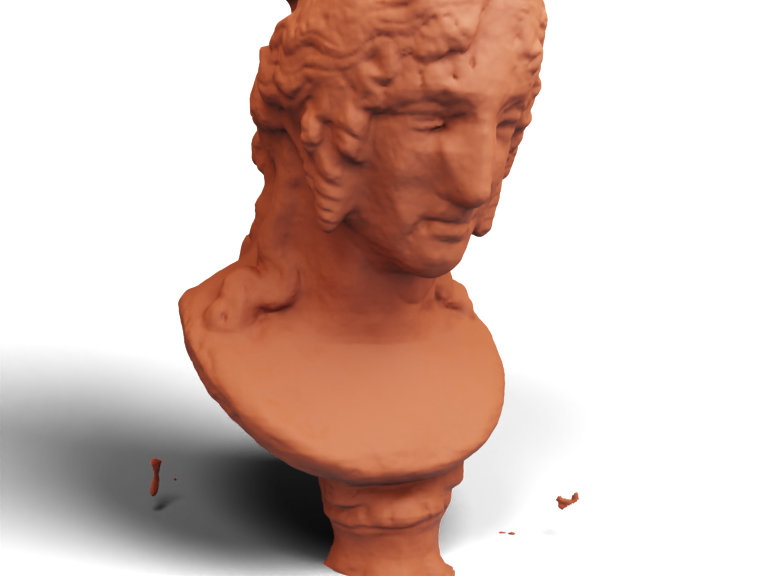
\includegraphics[width=0.3\linewidth]{figures/results/sculpture_neuralangelo.png} \\
        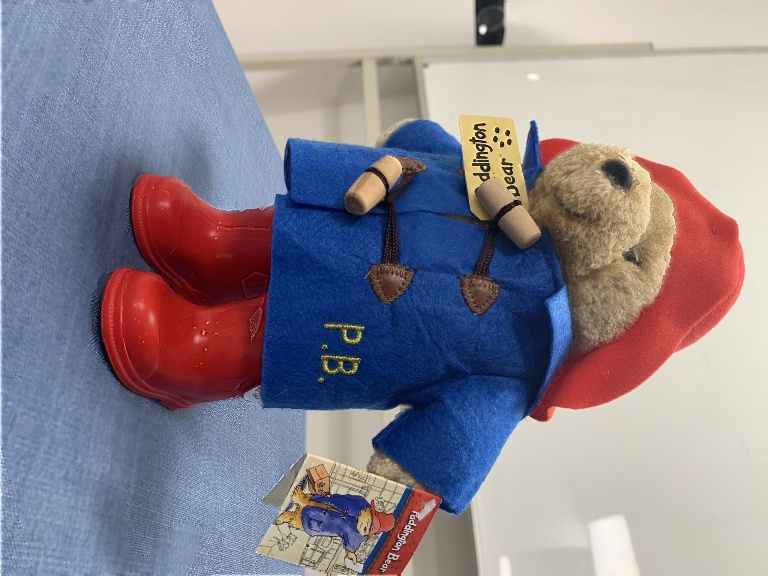
\includegraphics[width=0.3\linewidth]{figures/results/bear.png}
        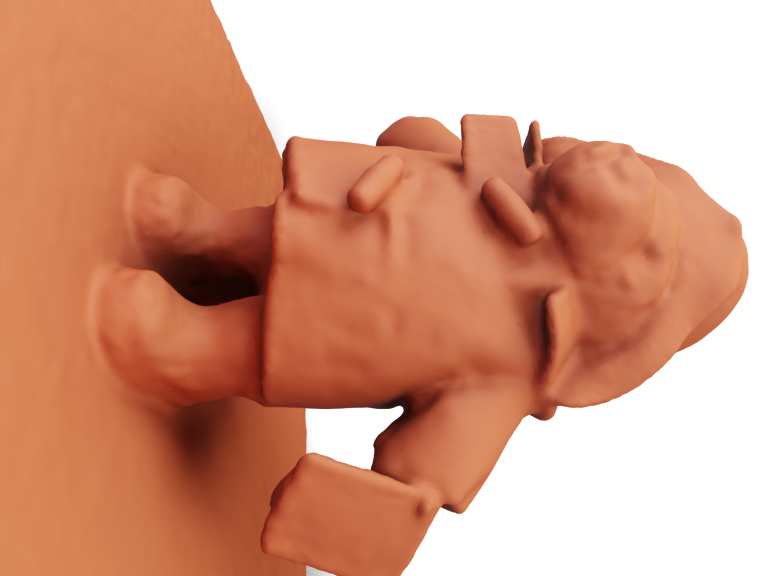
\includegraphics[width=0.3\linewidth]{figures/results/bear_ours.png}
        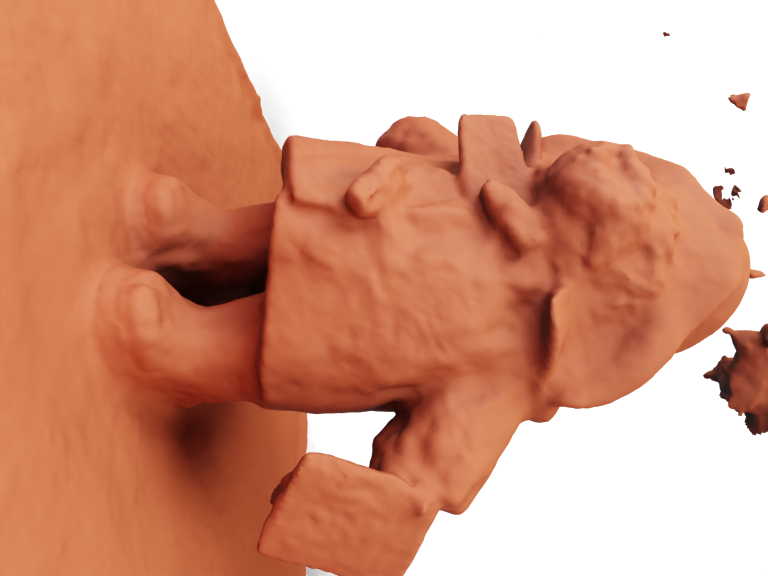
\includegraphics[width=0.3\linewidth]{figures/results/bear_neuralangelo.png} \\
        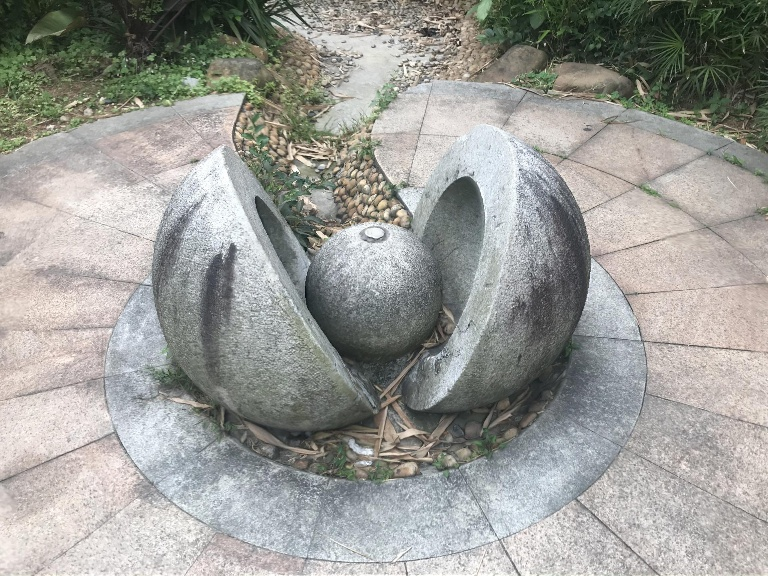
\includegraphics[width=0.3\linewidth]{figures/results/stone.png}
        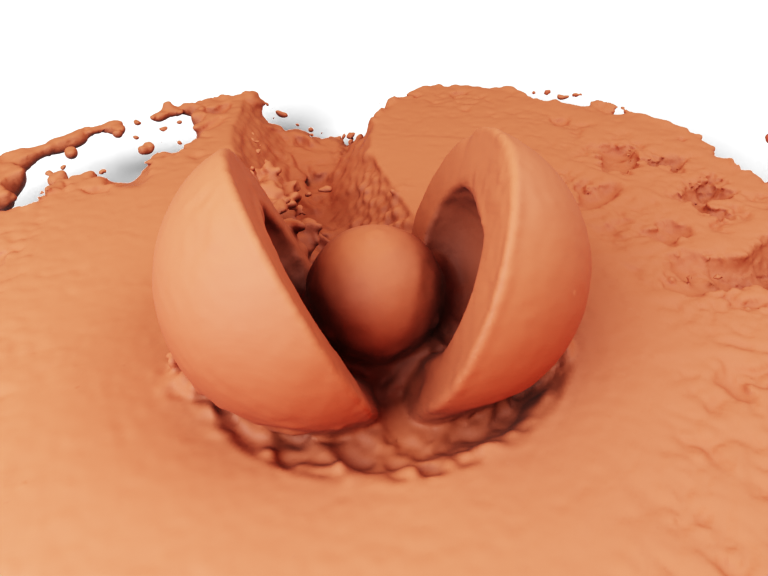
\includegraphics[width=0.3\linewidth]{figures/results/stone_ours.png}
        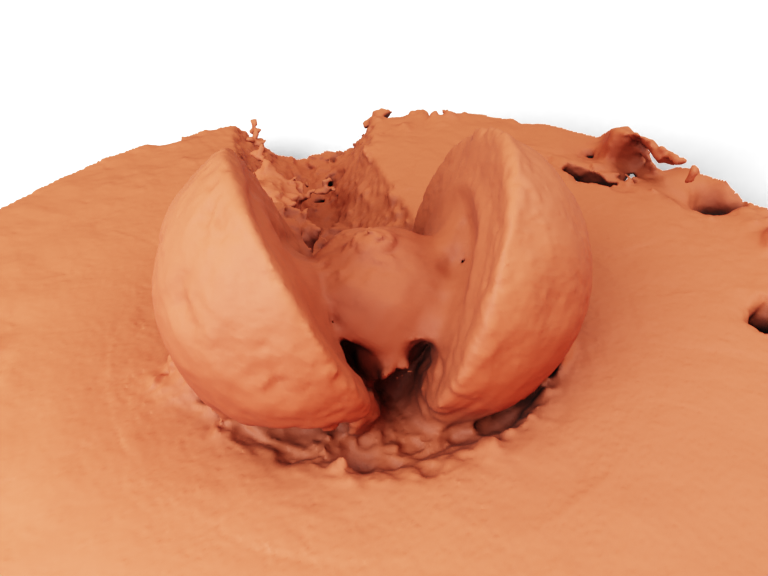
\includegraphics[width=0.3\linewidth]{figures/results/stone_neuralangelo.png}
    \end{figure}
\end{frame}

\begin{frame}{Results: \alert{BlendedMVS}}
    Neuralangelo completely fails when there are few views available:
    \begin{figure}
        \centering
        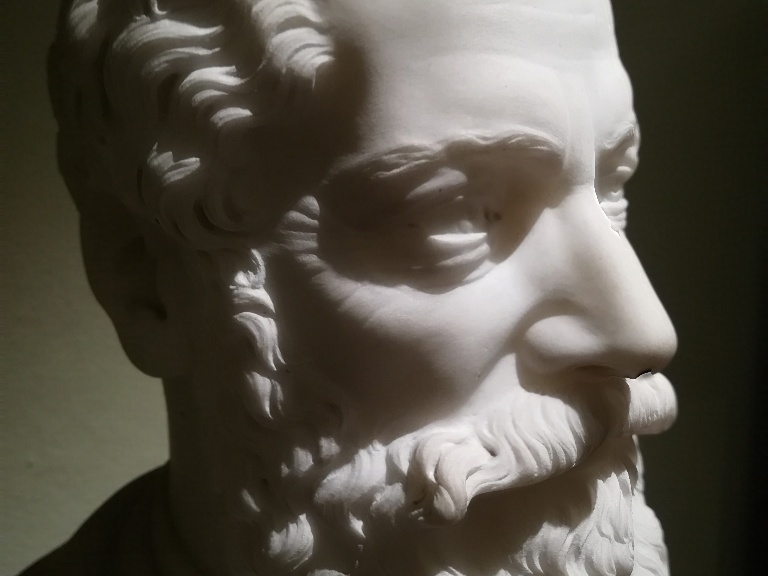
\includegraphics[width=0.3\linewidth]{figures/results/man.png}
        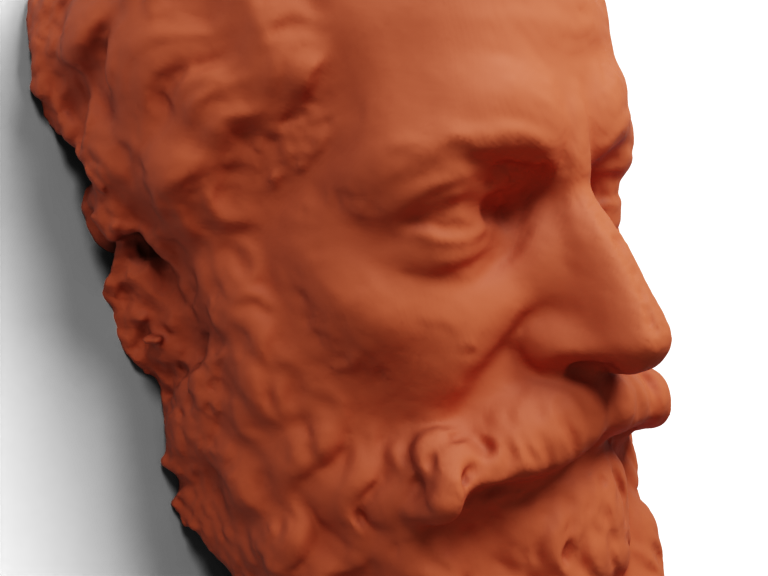
\includegraphics[width=0.3\linewidth]{figures/results/man_ours.png}
        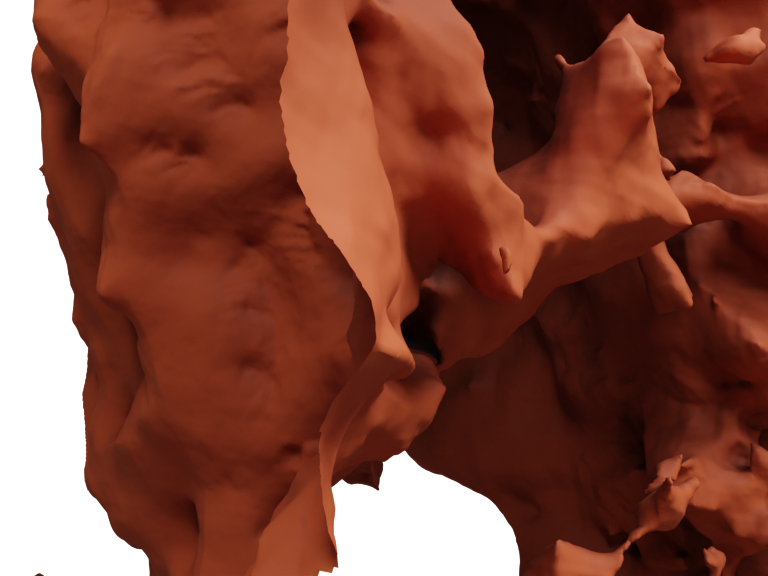
\includegraphics[width=0.3\linewidth]{figures/results/man_neuralangelo.png} \\
        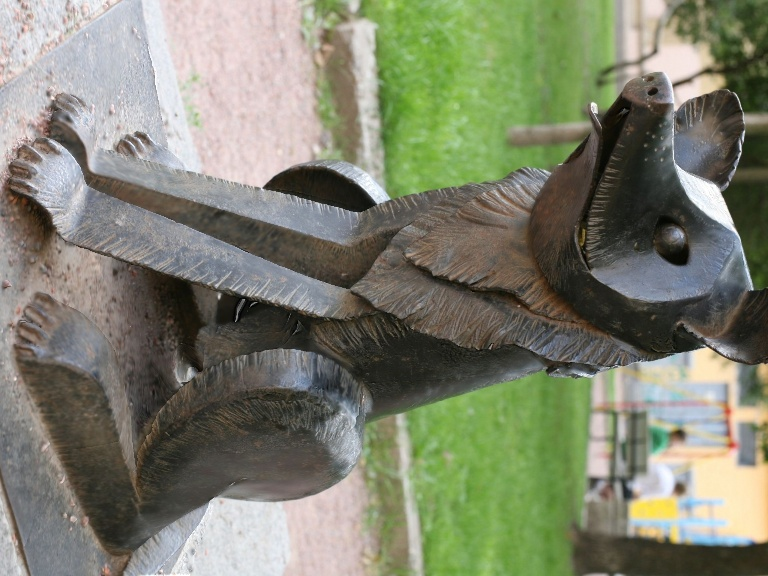
\includegraphics[width=0.3\linewidth]{figures/results/dog.png}
        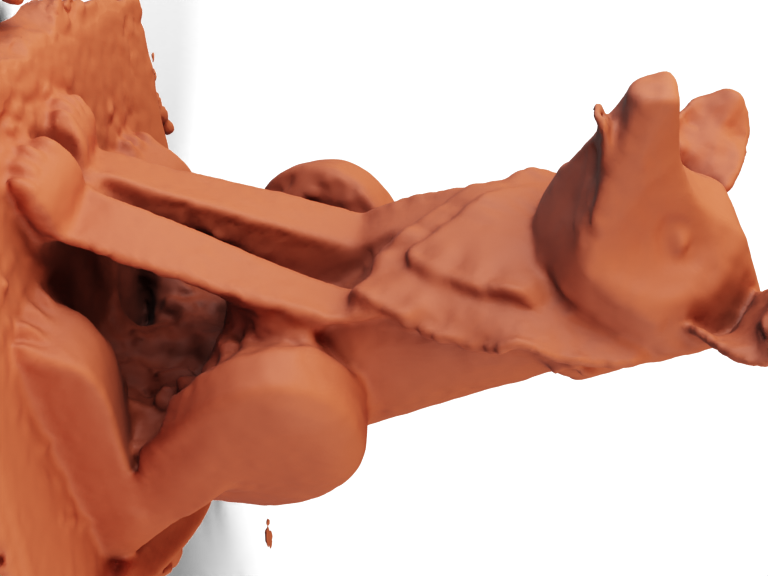
\includegraphics[width=0.3\linewidth]{figures/results/dog_ours.png}
        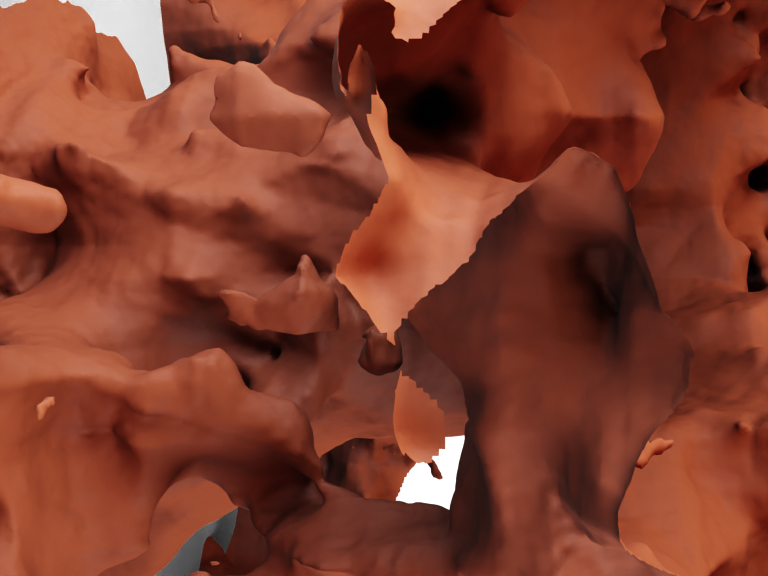
\includegraphics[width=0.3\linewidth]{figures/results/dog_neuralangelo.png}
    \end{figure}
\end{frame}

% \begin{frame}{Visualizations: \alert{Regularized} Dipole Sum}
%     We visualize the original winding number, the regularized winding number, and the regularized dipole sum (after training):
%     \begin{figure}
%         \centering
%         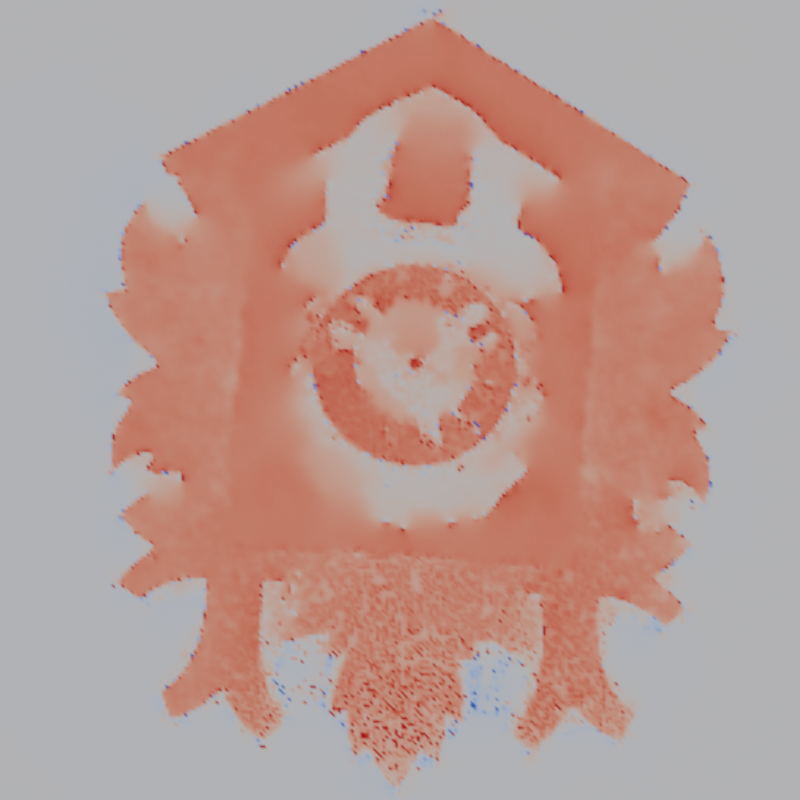
\includegraphics[width=0.3\linewidth]{figures/results/clock_wn_orig.png}
%         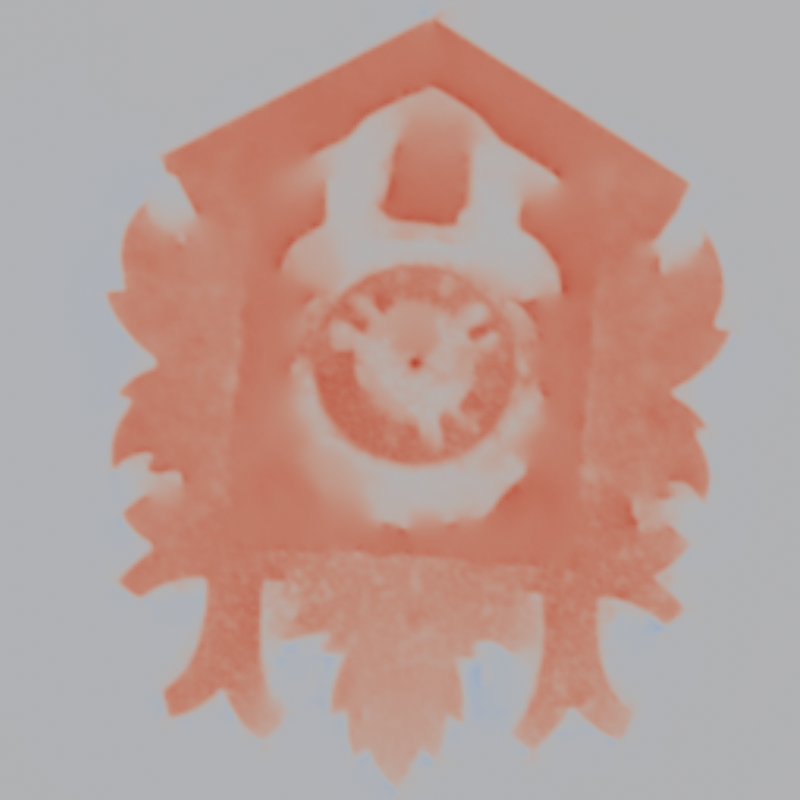
\includegraphics[width=0.3\linewidth]{figures/results/clock_wn_lin.png}
%         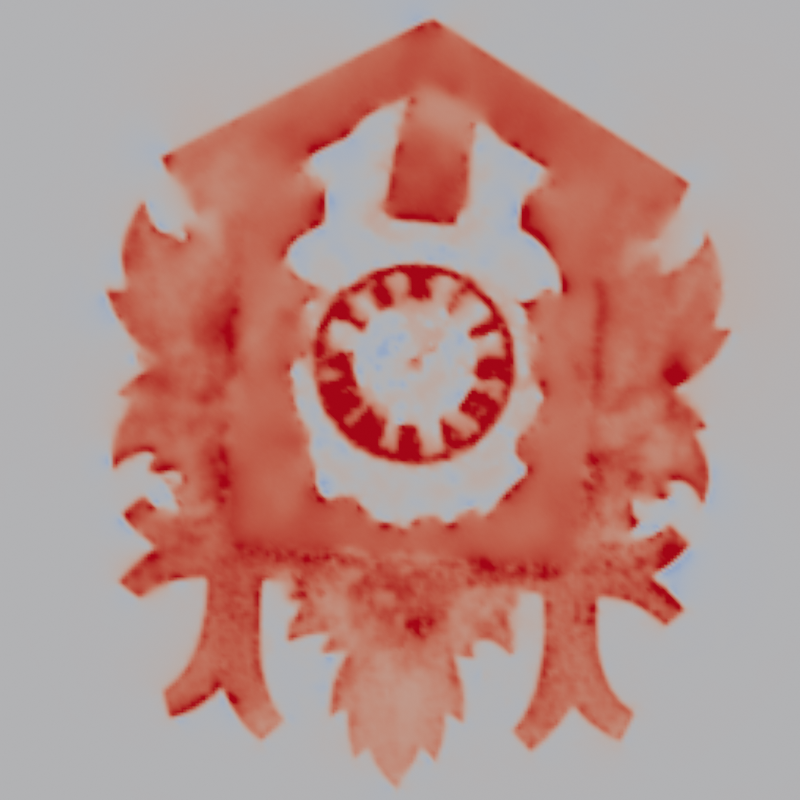
\includegraphics[width=0.3\linewidth]{figures/results/clock_wn_opt.png}
%     \end{figure}
% \end{frame}

\begin{frame}{Visualizations: Occupancy \& Color}
    We visualize the occupancy and color on slices of the scene:
    \begin{figure}
        \centering
        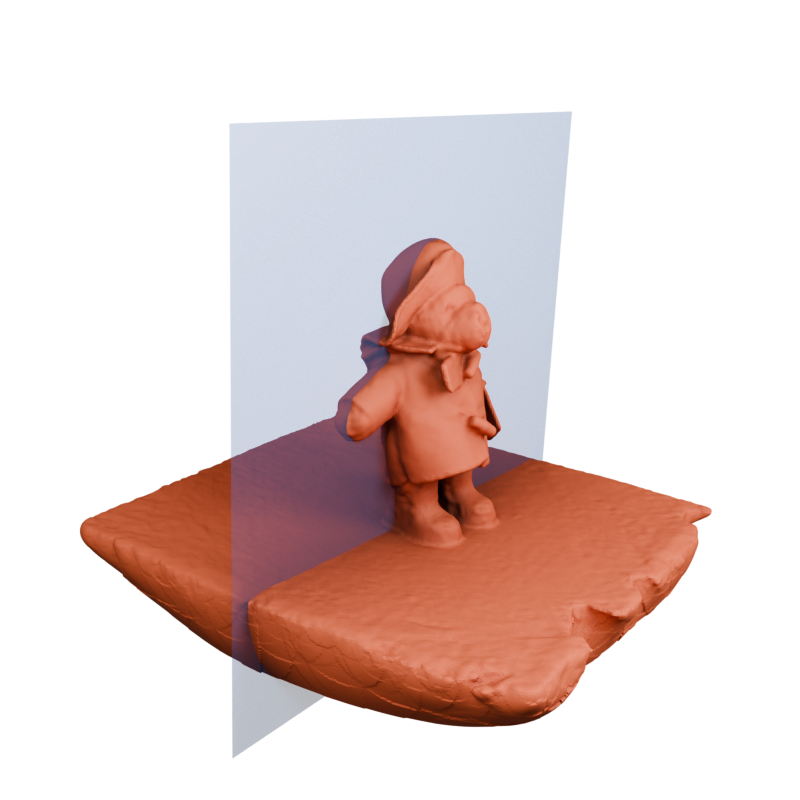
\includegraphics[width=0.3\linewidth]{figures/results/bear_plane.png}
        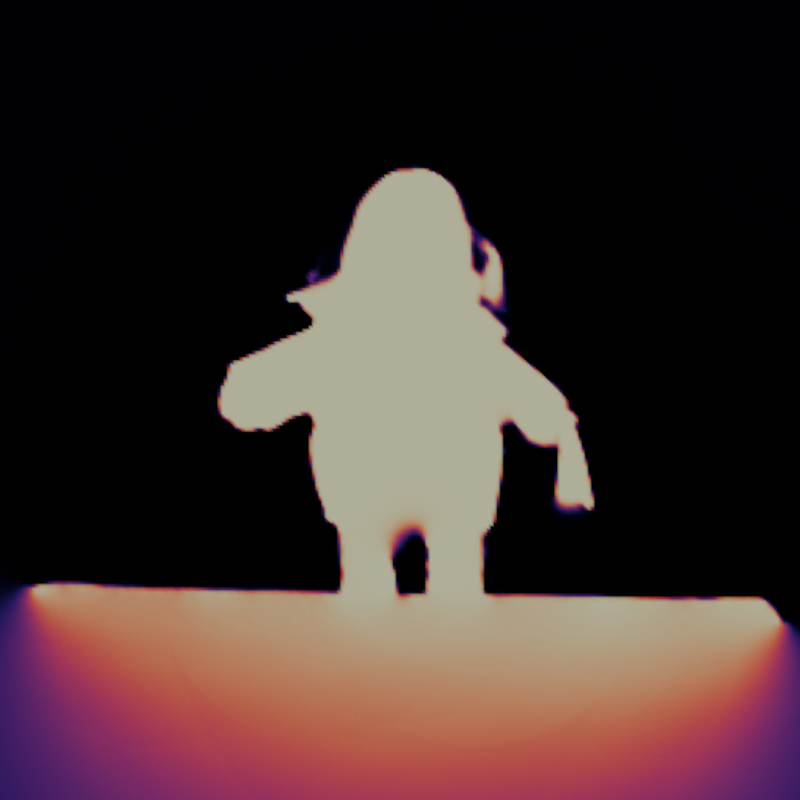
\includegraphics[width=0.3\linewidth]{figures/results/bear_occu.png}
        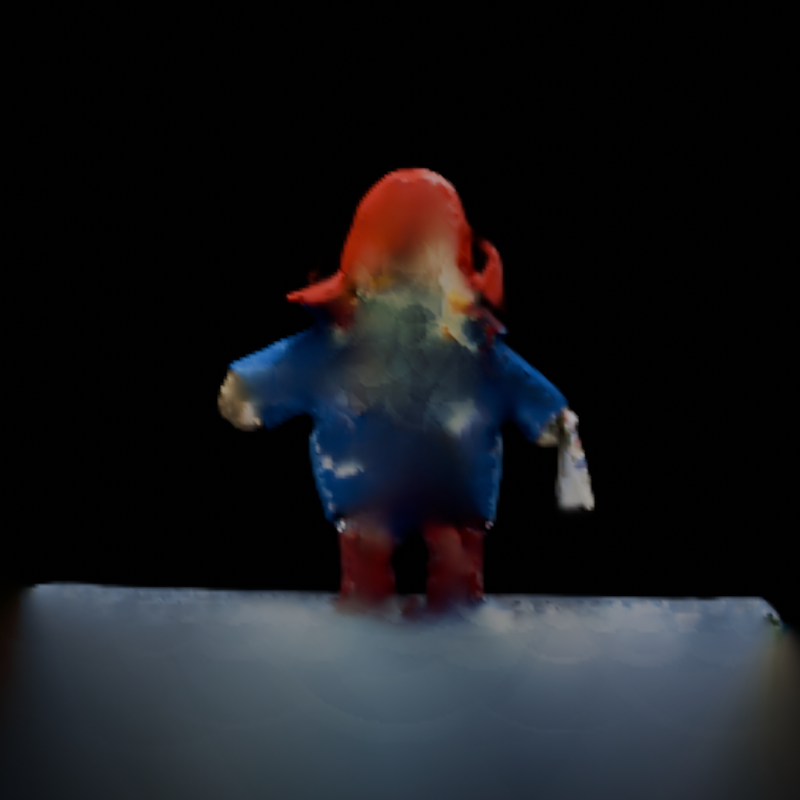
\includegraphics[width=0.3\linewidth]{figures/results/bear_color.png} \\\vspace{0.1em}
        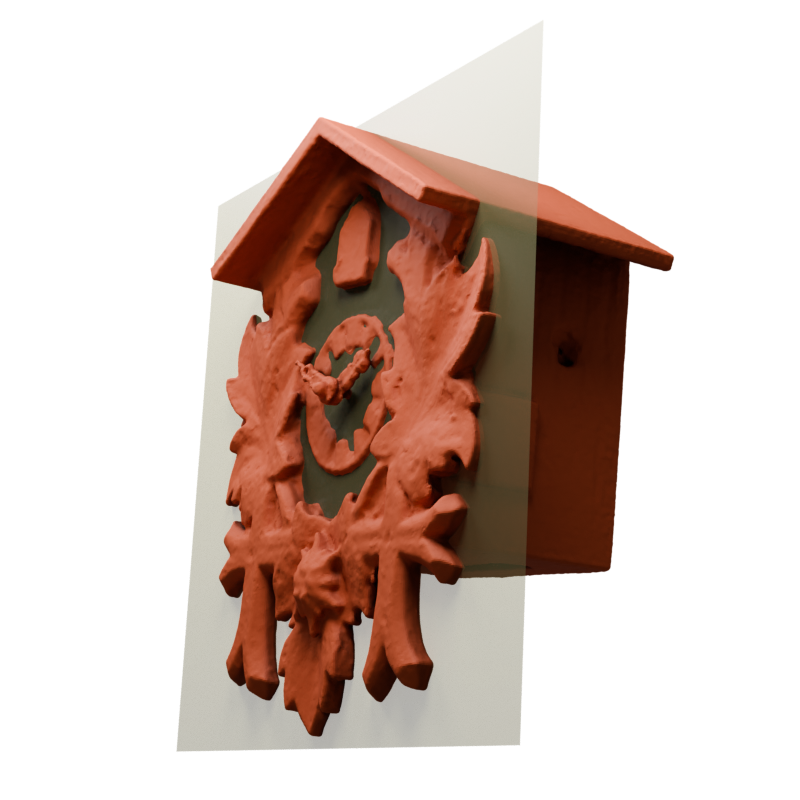
\includegraphics[width=0.3\linewidth]{figures/results/clock_plane.png}
        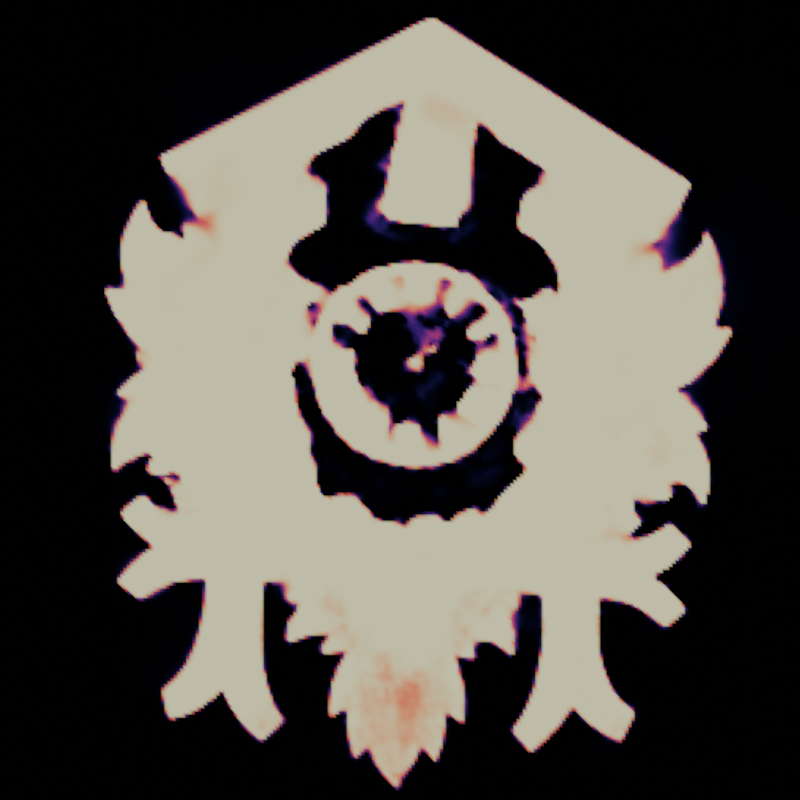
\includegraphics[width=0.3\linewidth]{figures/results/clock_occu.png}
        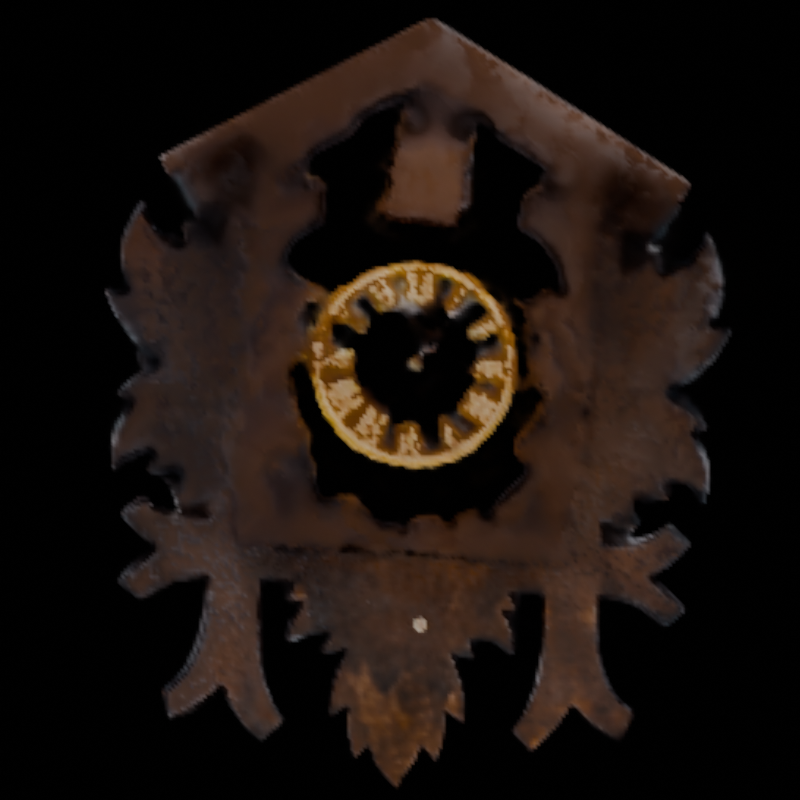
\includegraphics[width=0.3\linewidth]{figures/results/clock_color.png}
    \end{figure}
\end{frame}

\section{Conclusion}

\begin{frame}{Summary}
    We propose a novel method for 3D reconstruction that combines the \alert{efficiency} of point clouds (via the Barnes-Hut approximation) with the \alert{expressiveness} of neural rendering (via learnable boundary conditions and neural features).

    Our method achieves results comparable to the state-of-the-art in less than a quarter of the training time.

    Our representation is extremely \alert{compact}: the entire model consists of an oriented point cloud with a single additional scalar attribute at each point (< 50 MB).
\end{frame}

\begin{frame}{Limitations}
    Our reconstruction quality is highly dependent on the quality of the input point cloud, as we do not optimize point locations.

    For larger scale scenes, estimating a dense point cloud with Colmap can be a bottleneck for performance.

    Our method inherits certain limitations from Colmap, such as the difficulty in handling textureless surfaces and highly specular surfaces, where points are noisy or completely missing.
\end{frame}

\begin{frame}[standout]
    Questions?
\end{frame}

\begin{frame}[allowframebreaks]{References}
    \renewcommand{\bibsection}{}
    \bibliography{ref}
    \bibliographystyle{plainnat}
\end{frame}

\begin{frame}[standout]
    Thank you!
\end{frame}

\end{document}
